\title{PCB Analysis}

\date{\today}

\documentclass[12pt]{article}

\usepackage{graphicx}

\begin{document}
\maketitle

\section{Computational Hardware}

Ideally an inspection robot would be place in-between every step of the PCB manufacturing process. Since this would require potentially dozens of robots, creating a system that is cheap and scalable, would be ideal.  Because of this, all the software being developed in this project is being designed to work on the raspberry pi hardware.  This means that once one bot is fully developed and working on the raspberry pi, setting up another robot is as simple as copying an SD memory card. This allows for many bots to work in parallel while taking advantage of the economics of mass production. 

\newpage
\includegraphics[scale=0.1]{images/Computation_Resources/IMG_0620.JPG}

Inspection bot software running on a raspberry pi.  It has just enough cpu power to control both the printer and perform PCB image analysis.  
\newpage
\includegraphics[scale=0.1,angle=270]{images/Computation_Resources/IMG_0619.JPG}

Uses a very cheap USB microscope.  Although a higher end one would be necessary for detailed volume analysis of board components. 

\newpage
\includegraphics[scale=0.1]{images/Computation_Resources/IMG_0621.JPG}

The usb microscope and printer are run off of the raspberry pi using a powered usb hub.  This is not an ideal way to capture image data since running a camera over the raspberry pi usb port is very slow.  Ideally the system would use the raspberry pi camera to take images since the raspberry pi camera connect directly to the raspberry pi bus.  But this would require adding a lens to the raspberry pi camera in order to change it into a microscope.   

\newpage
\includegraphics[scale=0.1]{images/Computation_Resources/IMG_0622.JPG}

An image of the inspection bot software running on the raspberry pi. 
\section{Printer Path}
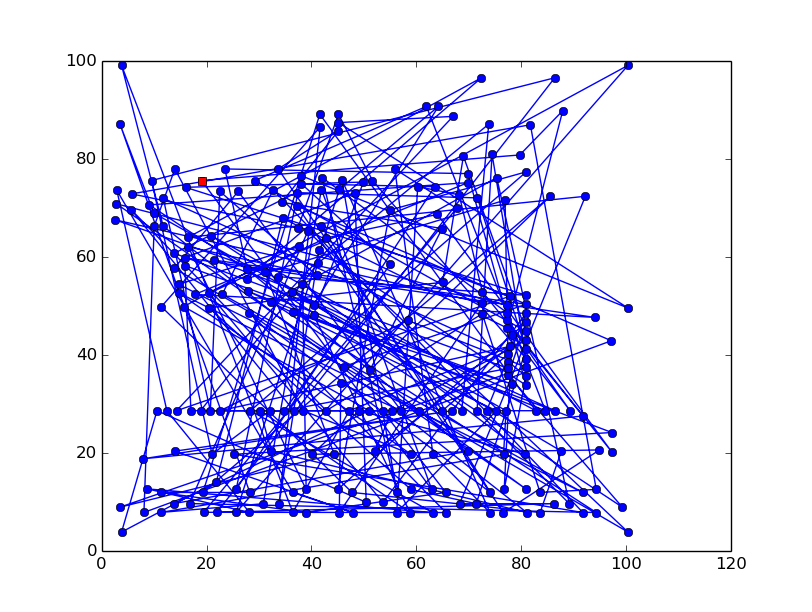
\includegraphics[scale=0.8]{images/Path/original_path.png}

original path from PCB component list. 
\newpage
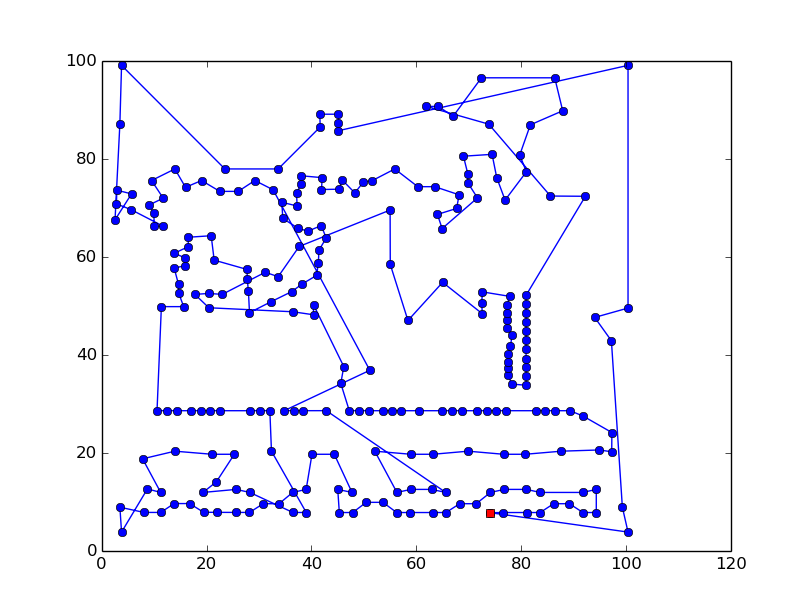
\includegraphics[scale=0.8]{images/Path/best_found_path.png}

By finding a more efficient path, as seen above, the time required to scan all the components on a chip goes from a half an hour to less than 3 mins. 

\section{Chip Analysis Setup}
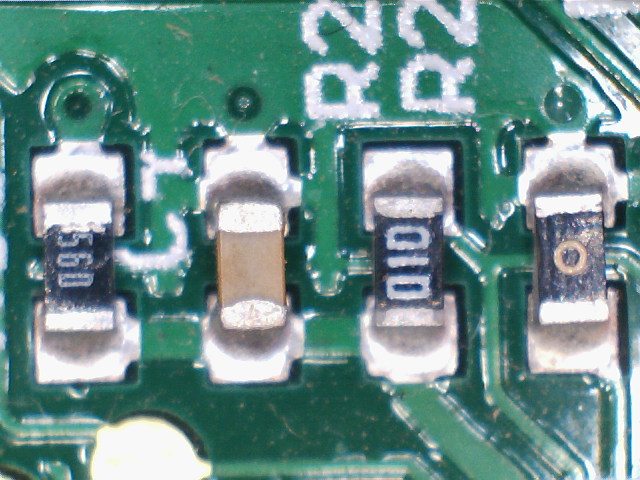
\includegraphics[scale=0.8]{images/Segmentation/raw_image.png}

Most components on a PCB board have a unique color signature.  By detecting this signature it is possible to detect and track components as the bot moves. 

\newpage
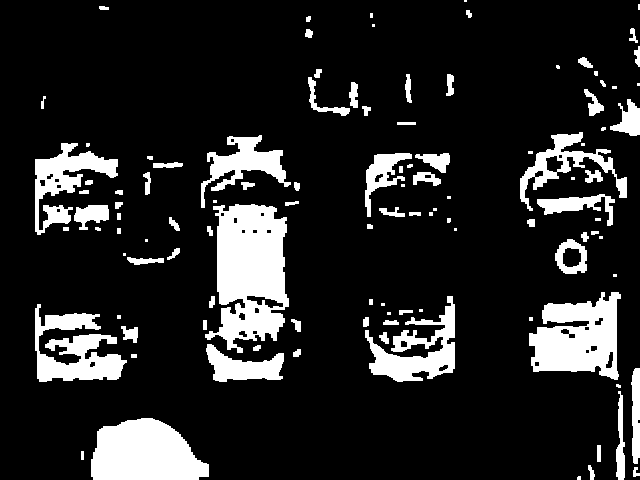
\includegraphics[scale=0.8]{images/Segmentation/binary.png}
\newpage
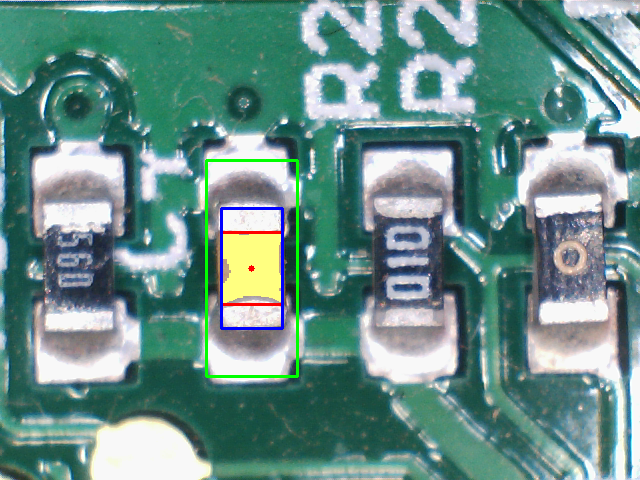
\includegraphics[scale=0.8]{images/Segmentation/part_analysis.png}


\section{Volume Analysis Setup}
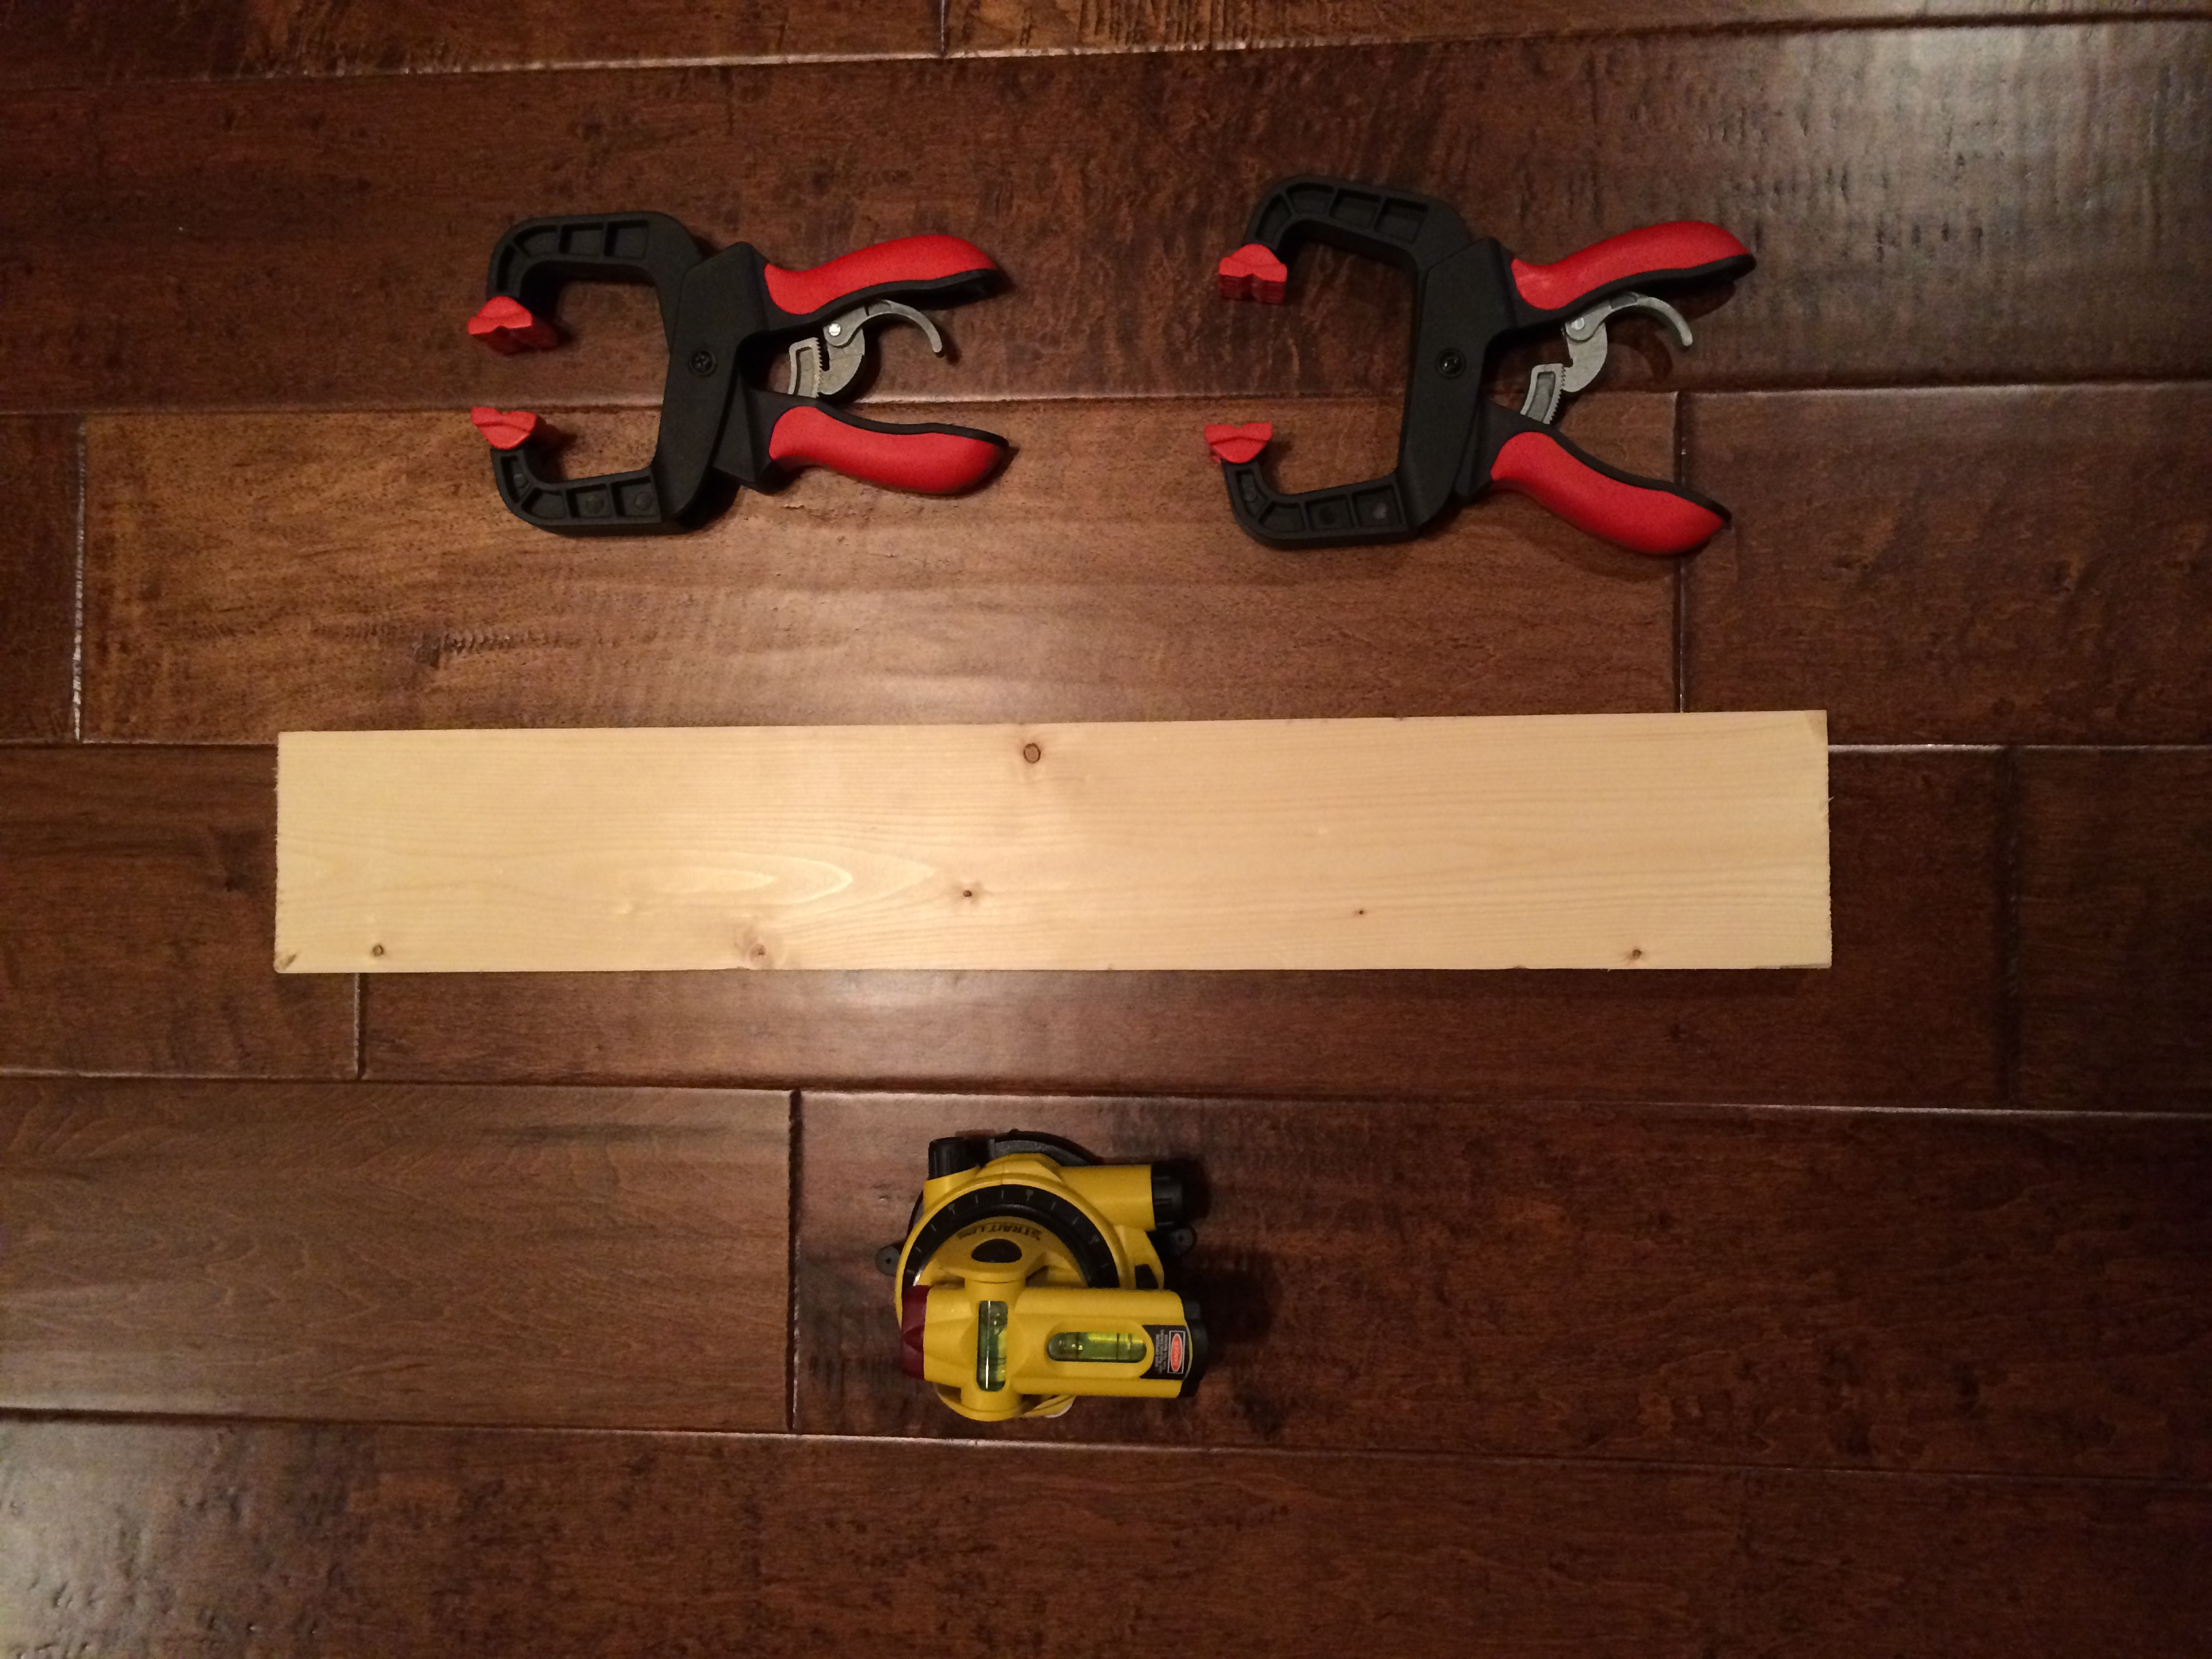
\includegraphics[scale=0.1,angle=270]{images/volume_analysis_setup/IMG_0618.JPG}
\newpage
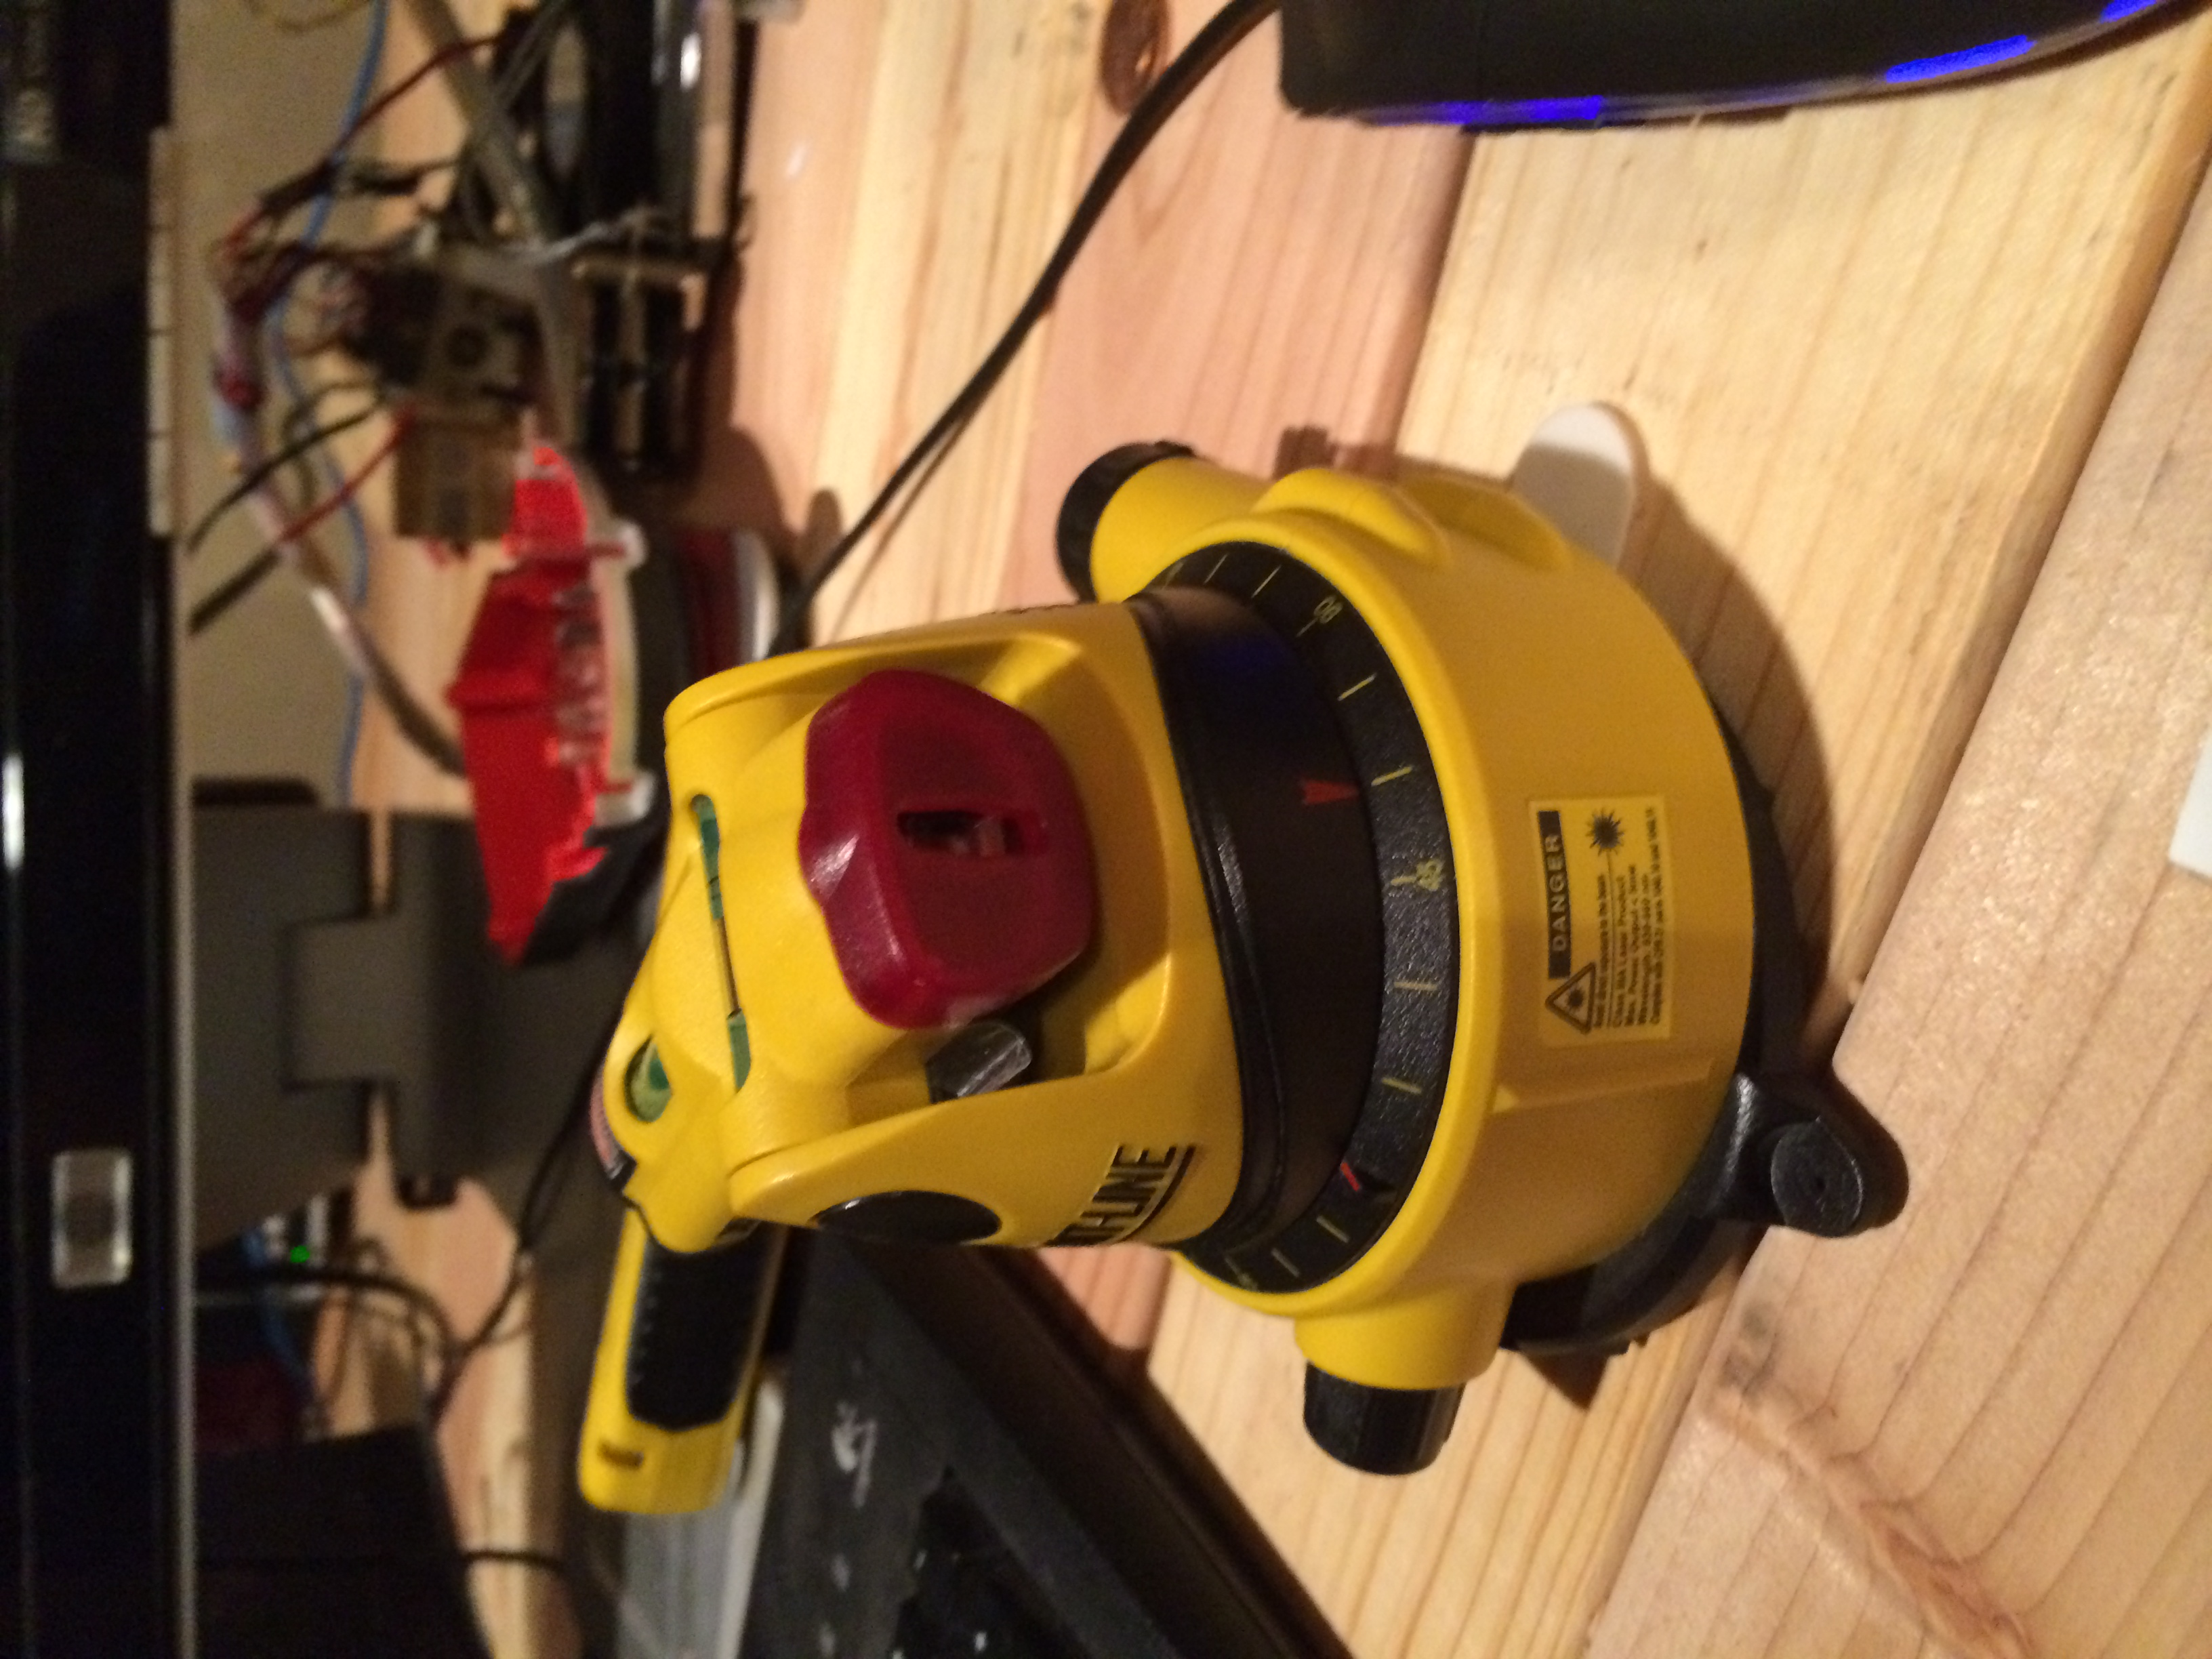
\includegraphics[scale=0.1,angle=270]{images/volume_analysis_setup/IMG_0616.JPG}
\newpage
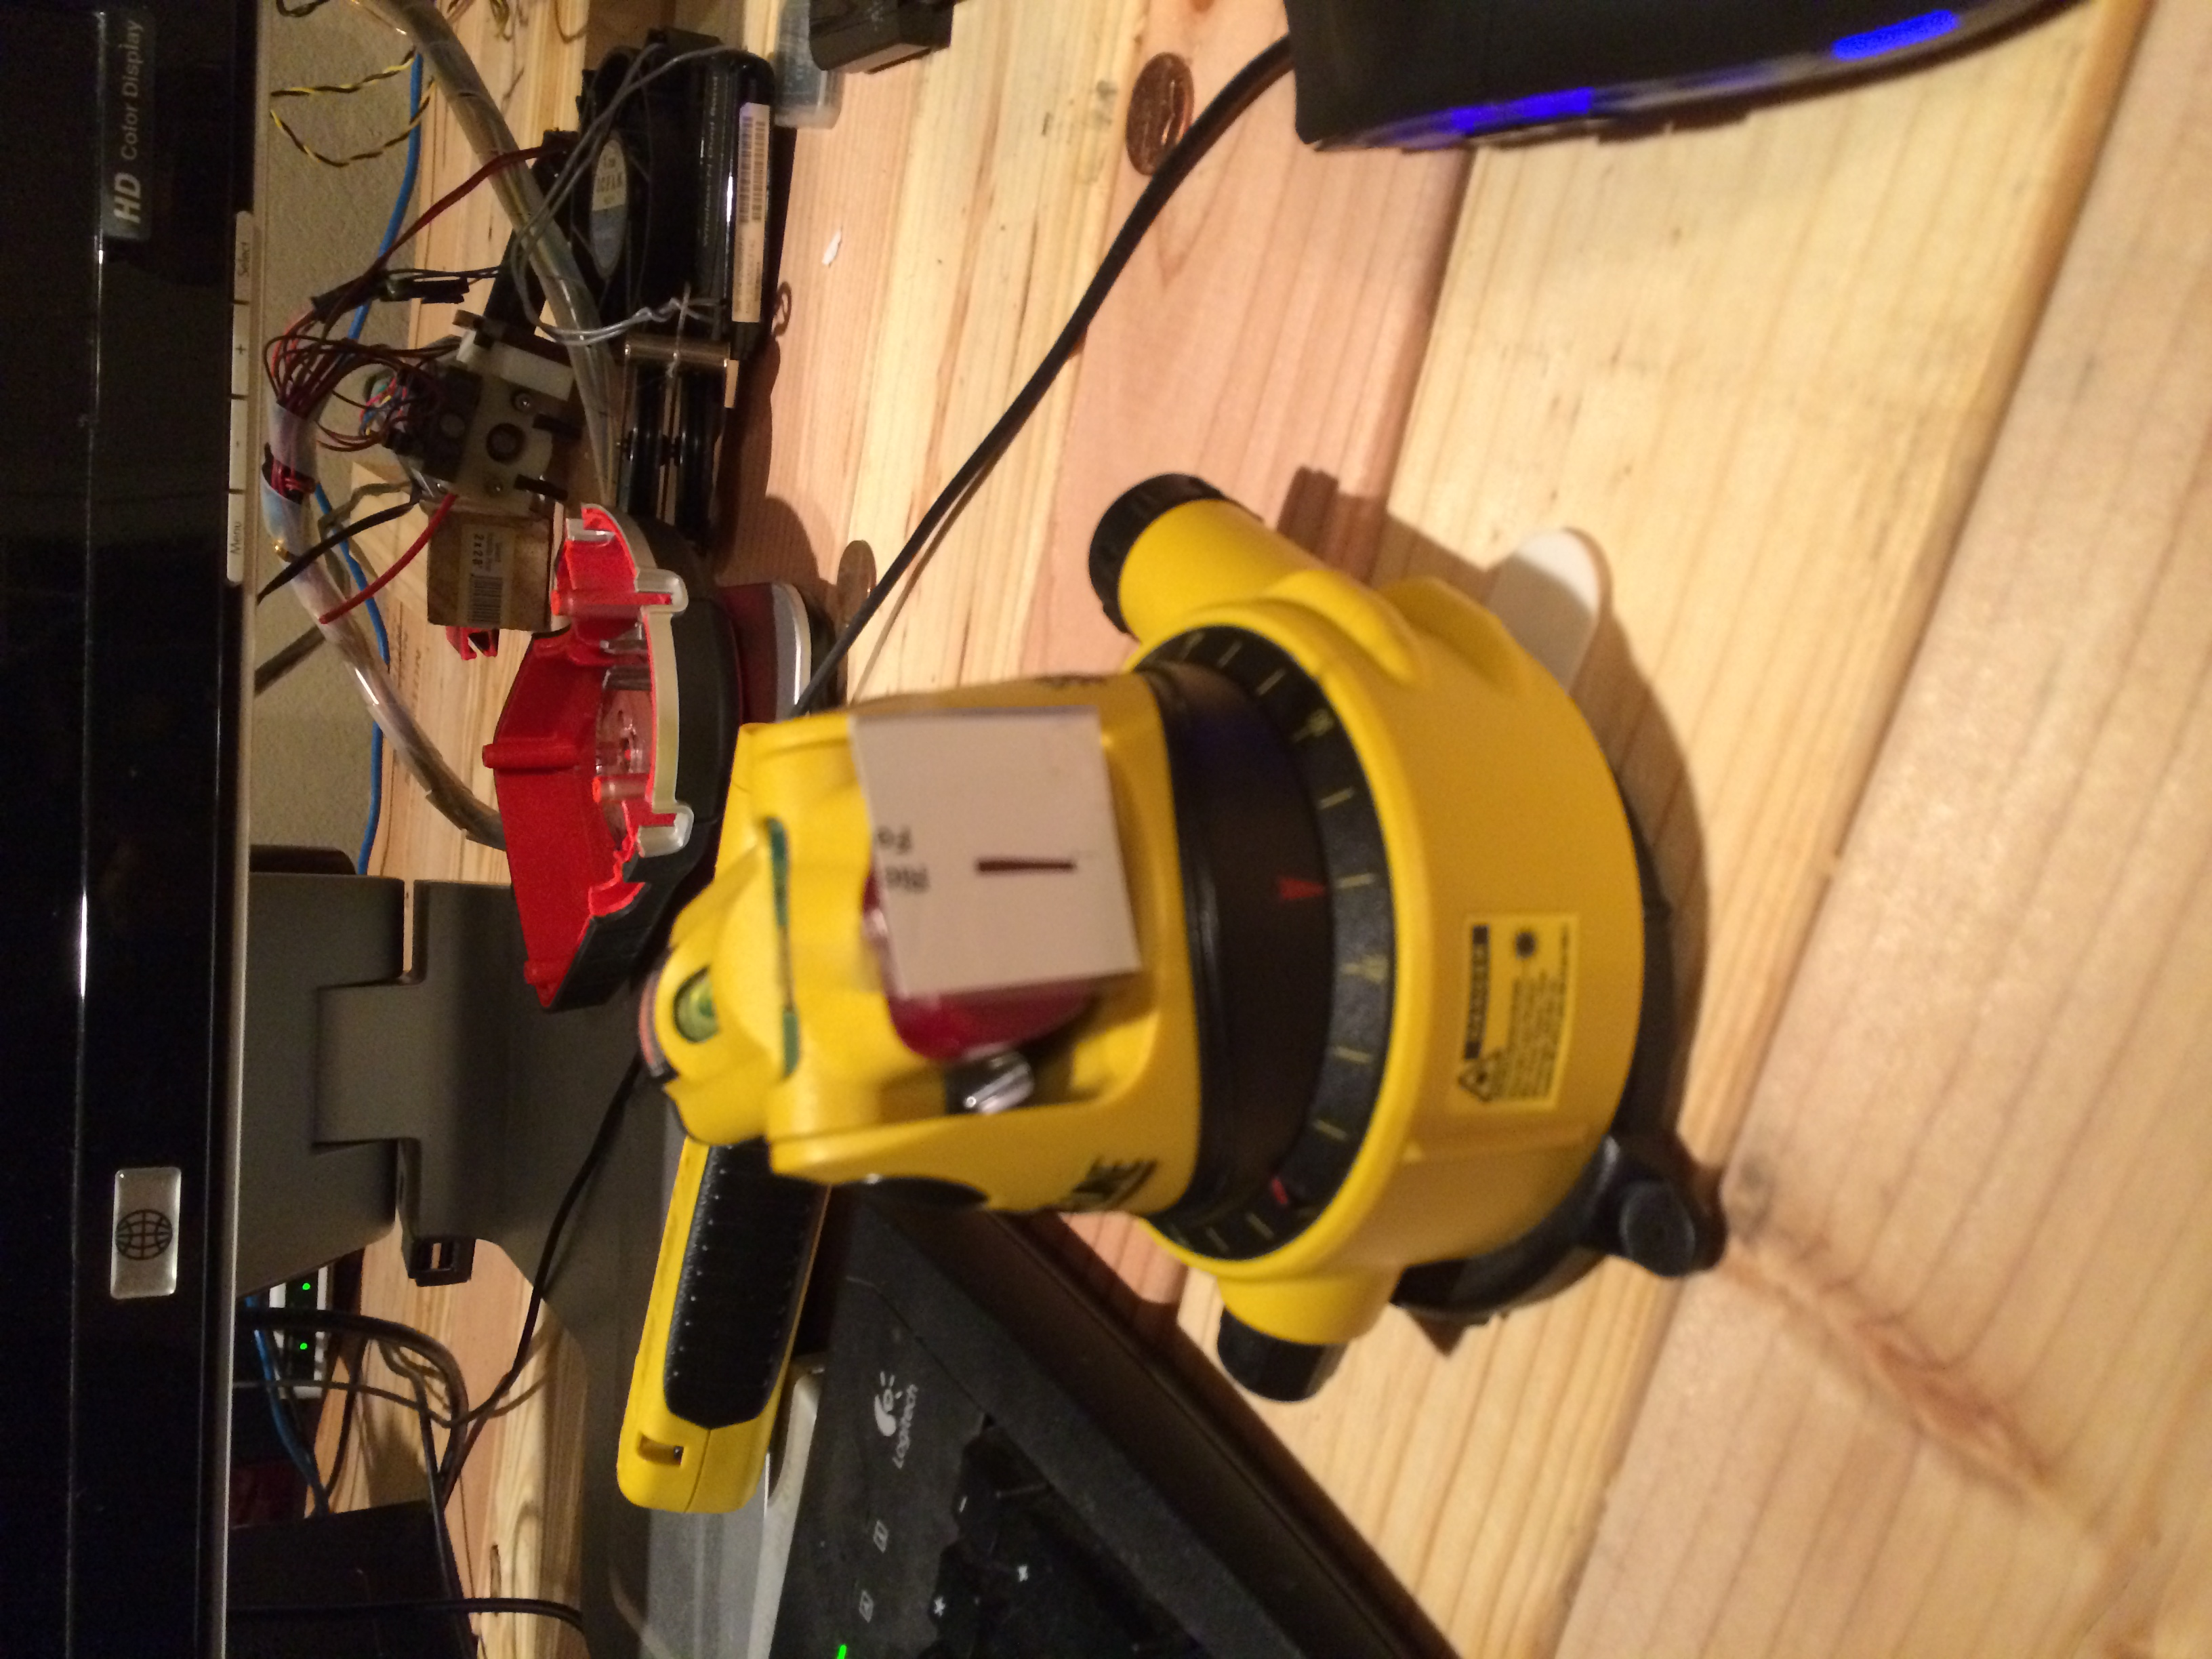
\includegraphics[scale=0.1,angle=270]{images/volume_analysis_setup/IMG_0617.JPG}
\newpage
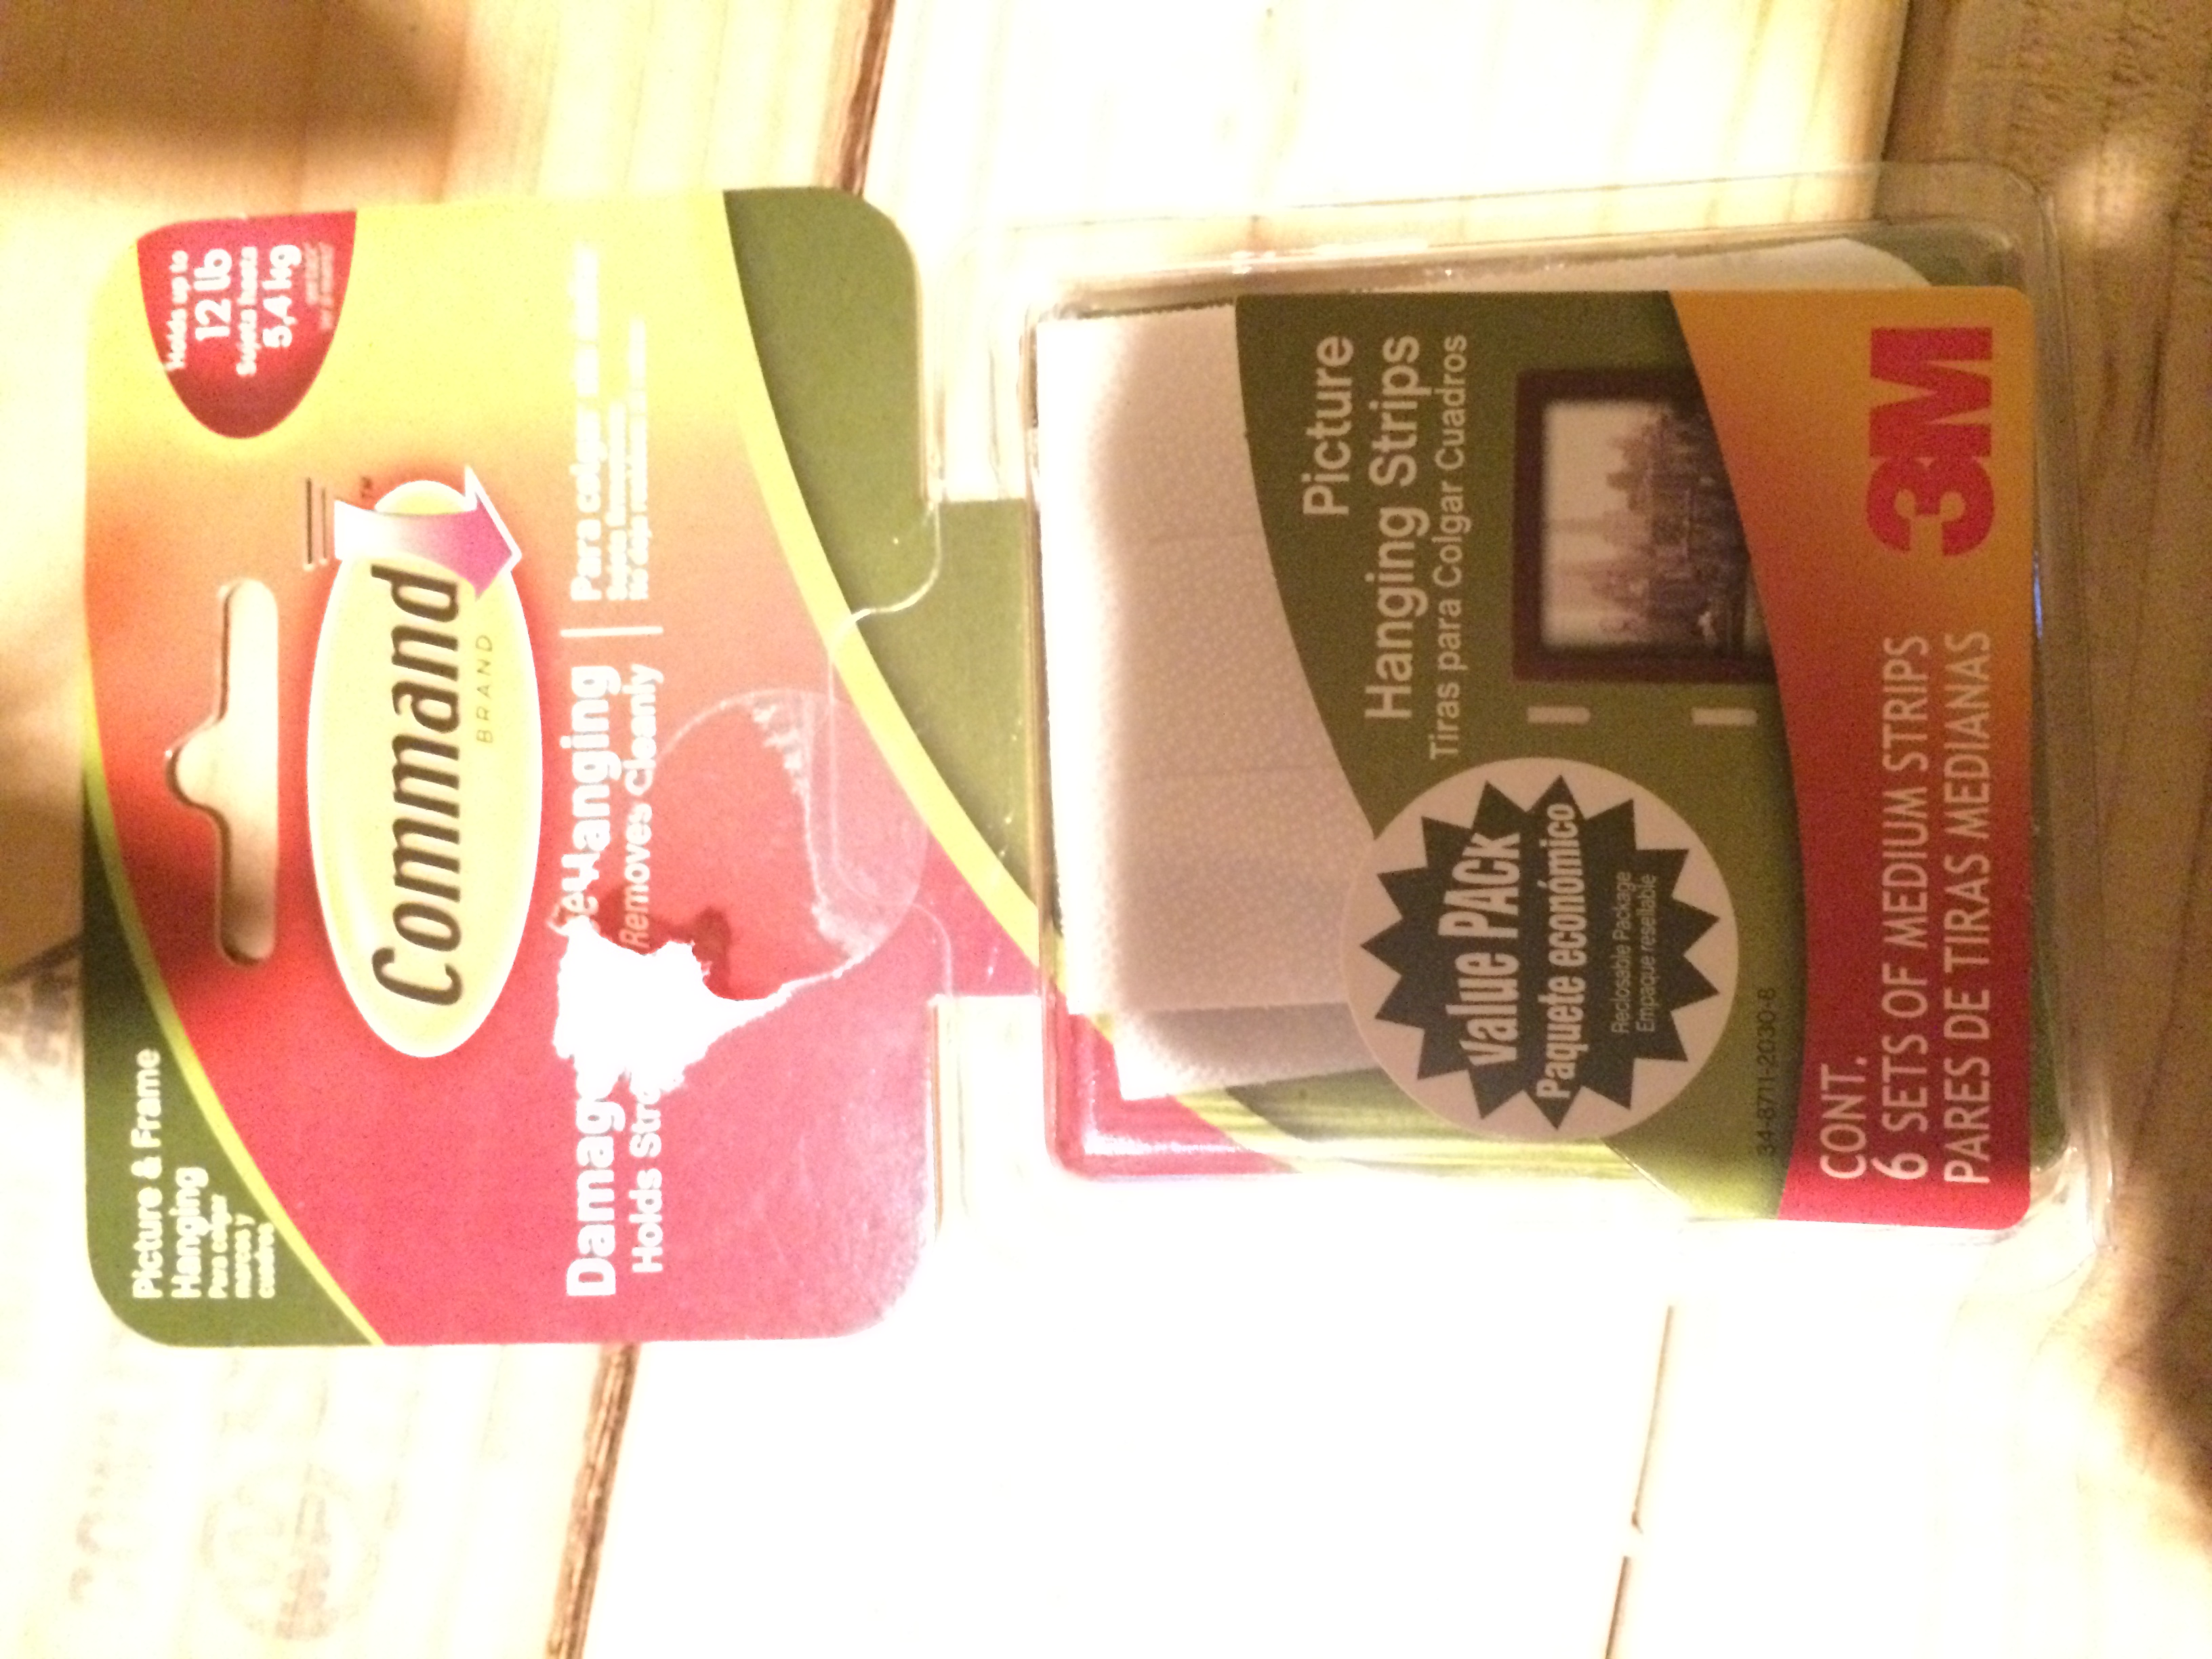
\includegraphics[scale=0.1,angle=270]{images/volume_analysis_setup/IMG_0613.JPG}
\newpage
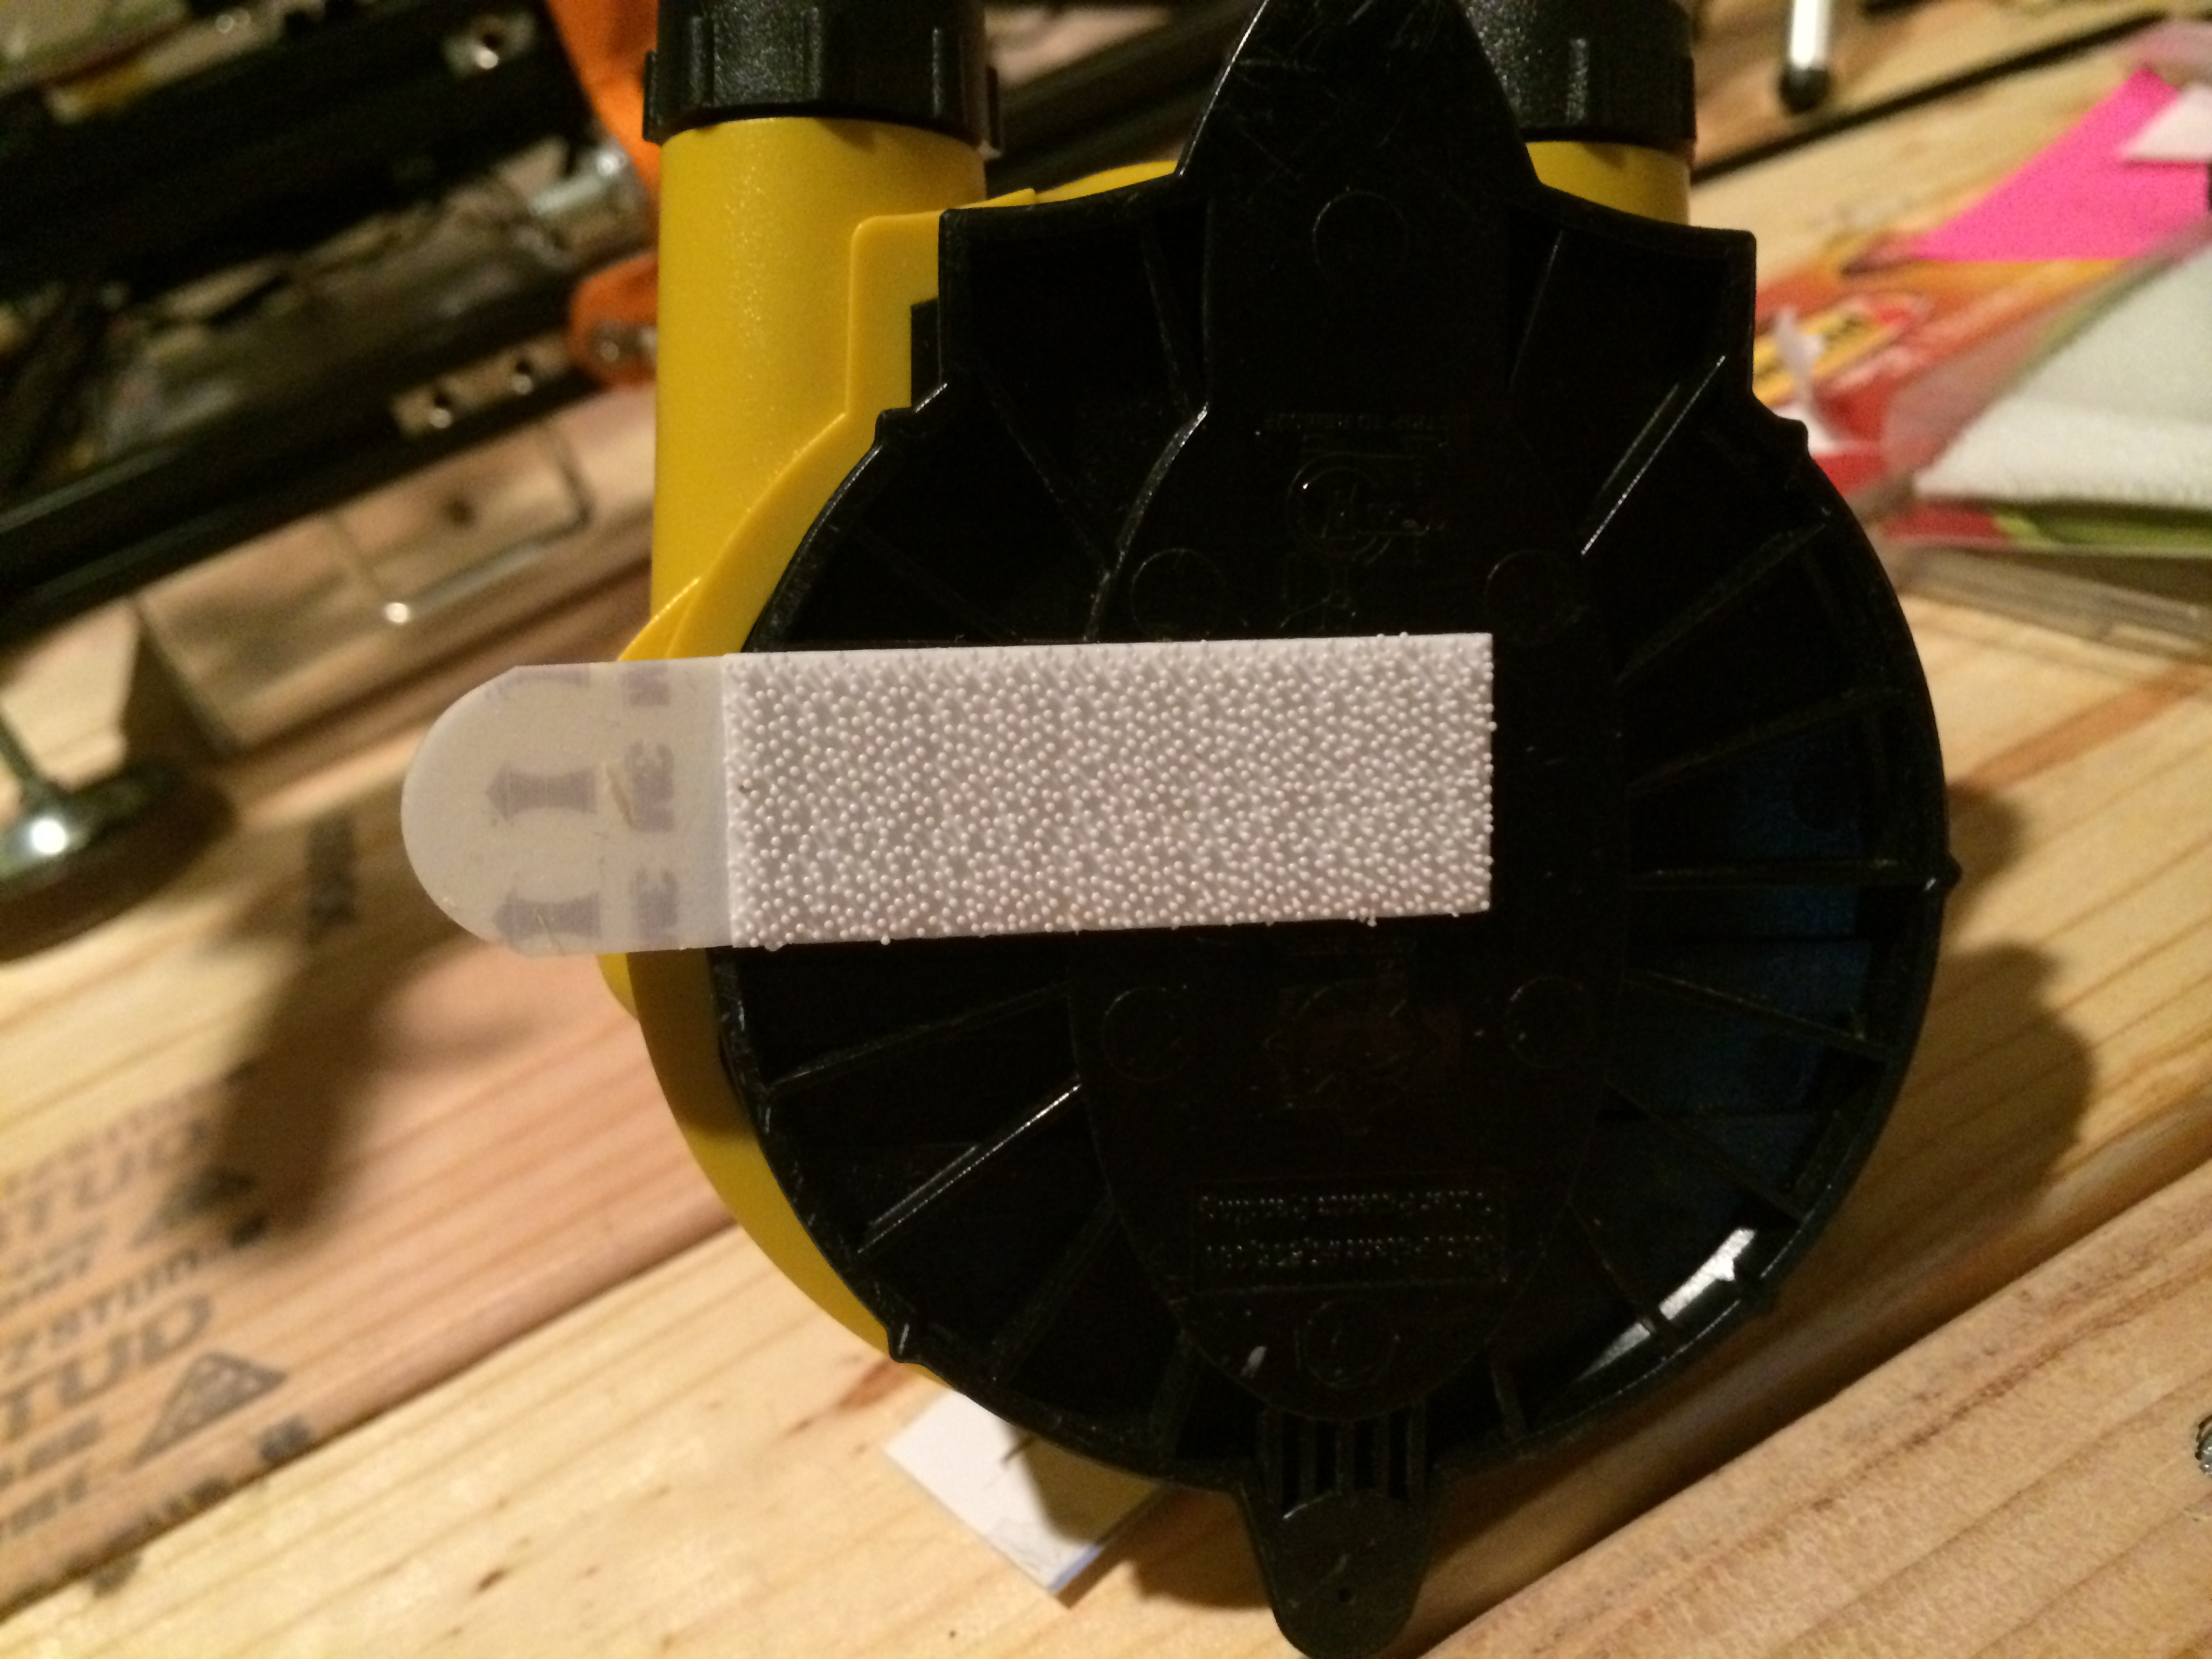
\includegraphics[scale=0.1,angle=270]{images/volume_analysis_setup/IMG_0611.JPG}
\newpage
%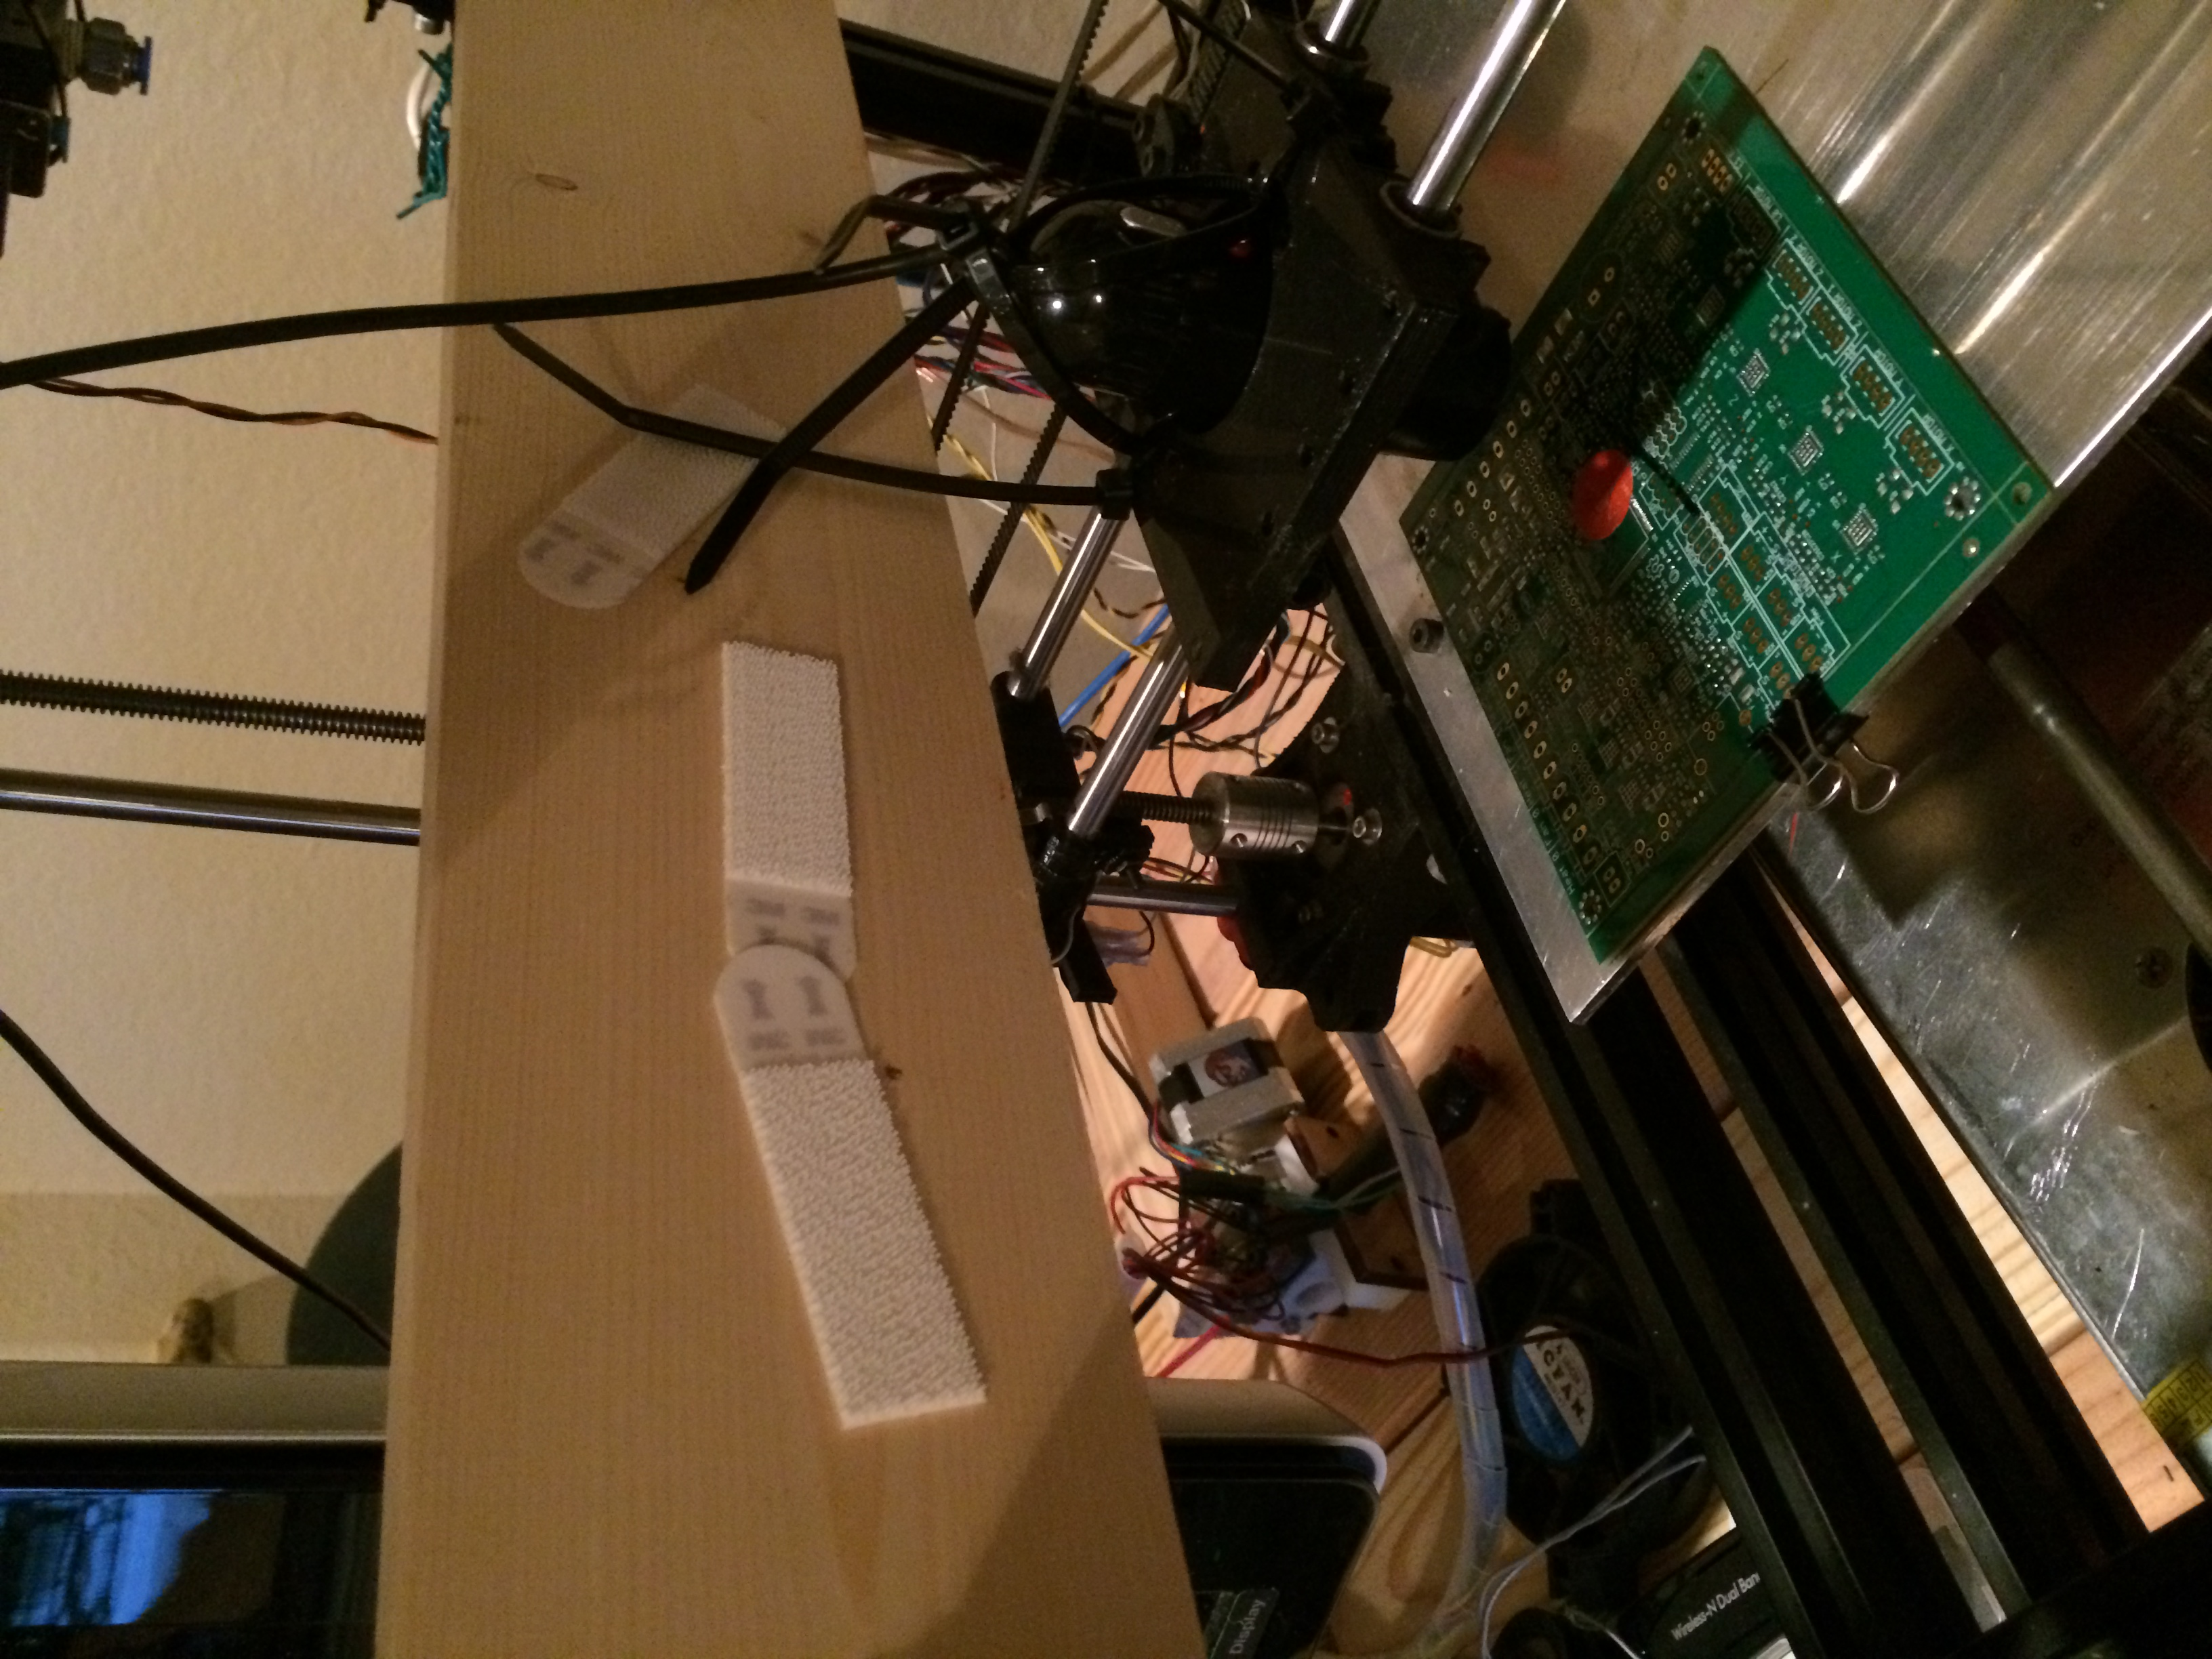
\includegraphics[scale=0.1,angle=270]{images/volume_analysis_setup/IMG_0612.JPG}
%\newpage
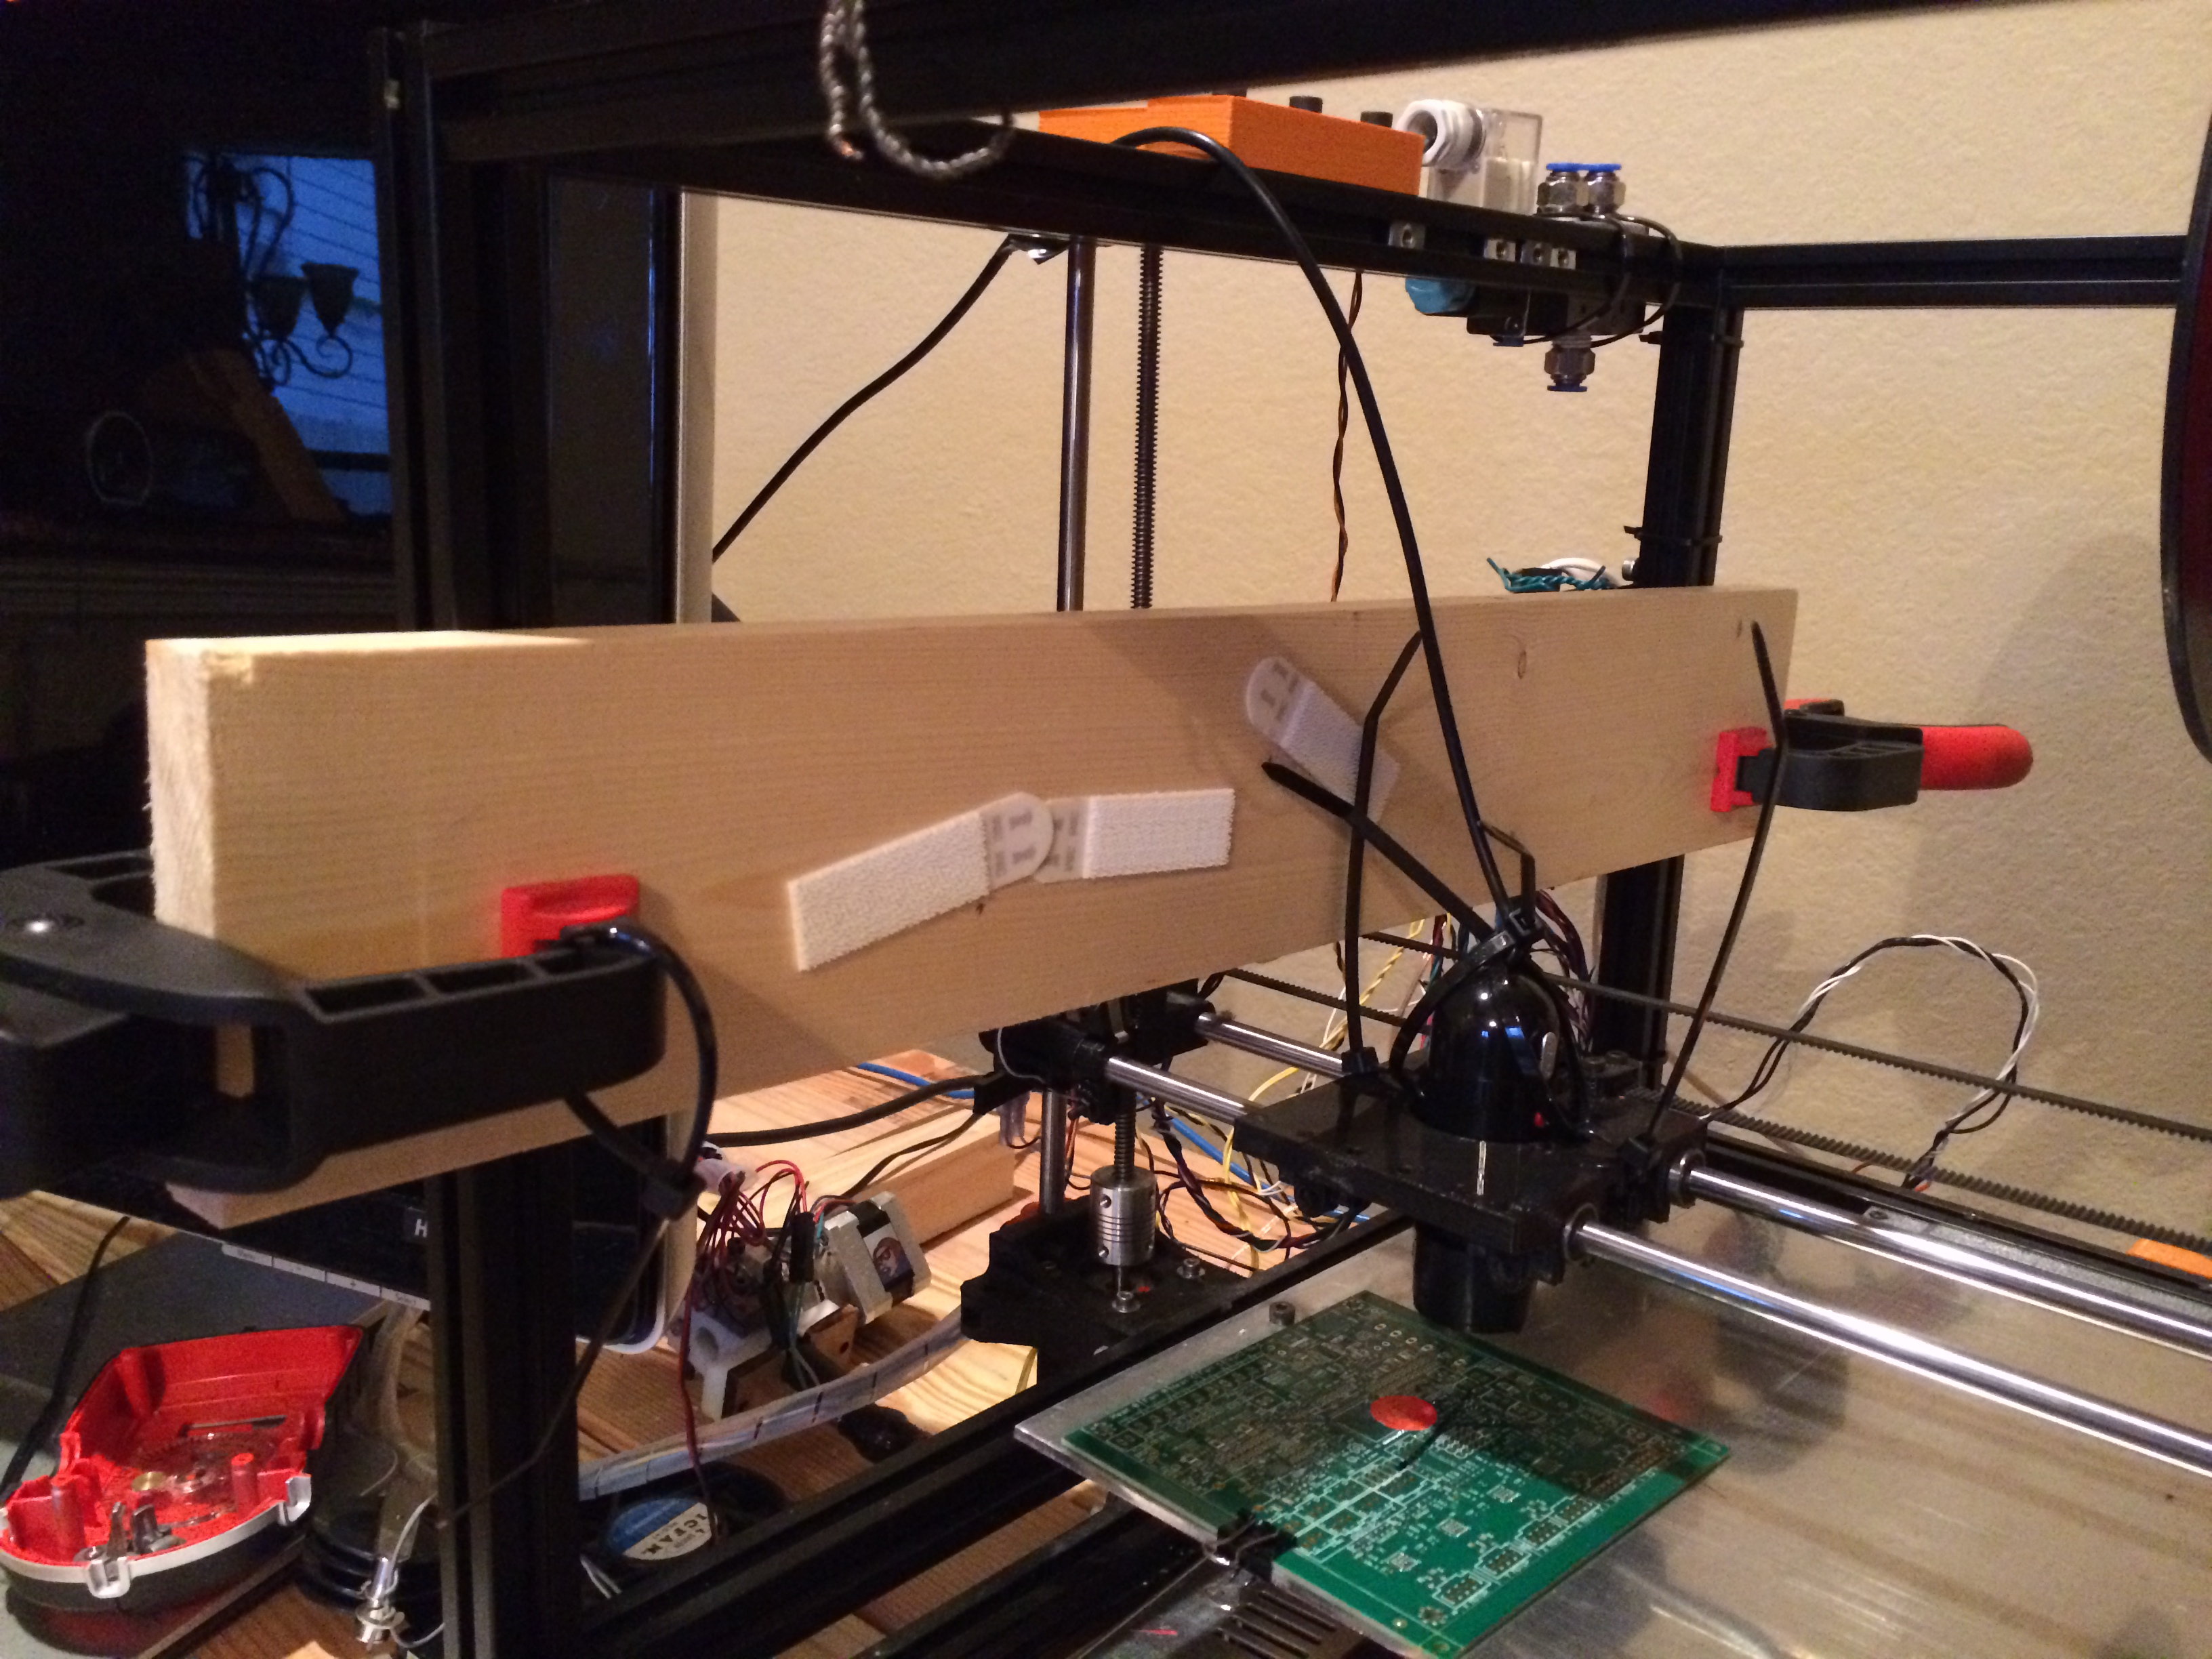
\includegraphics[scale=0.1]{images/volume_analysis_setup/IMG_0614.JPG}
\newpage

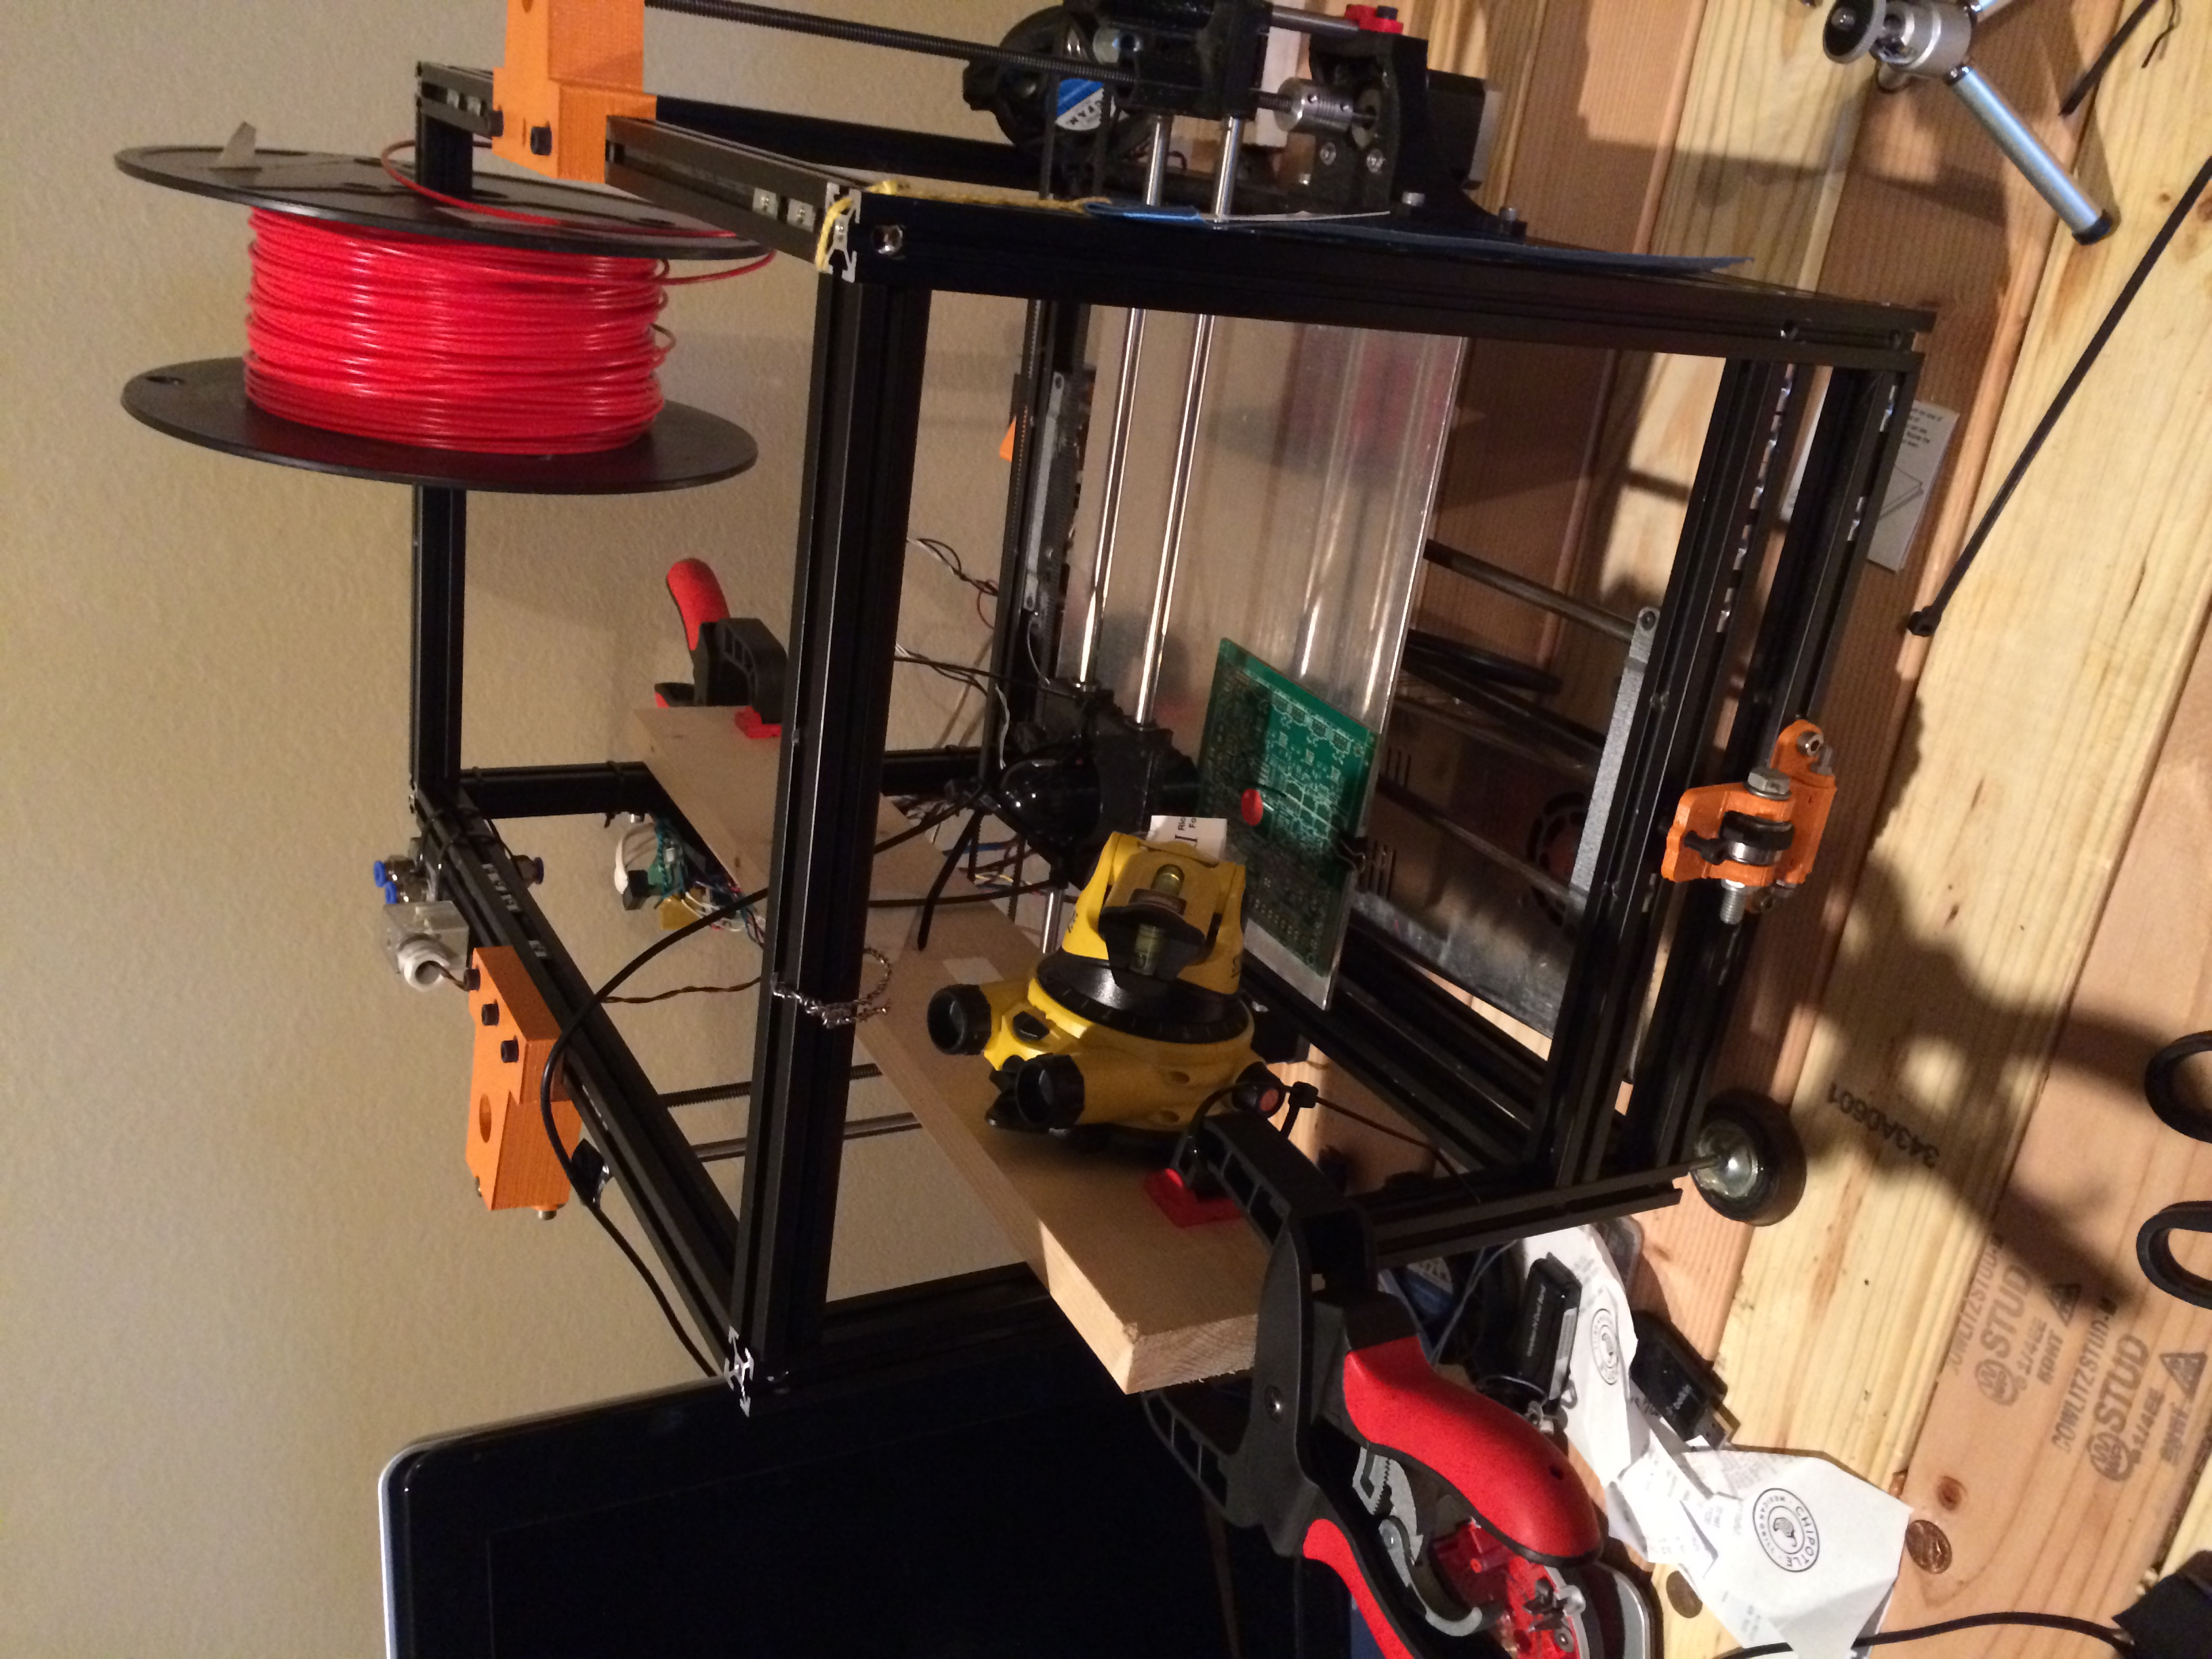
\includegraphics[scale=0.1,angle=270]{images/volume_analysis_setup/IMG_0604.JPG}
\newpage
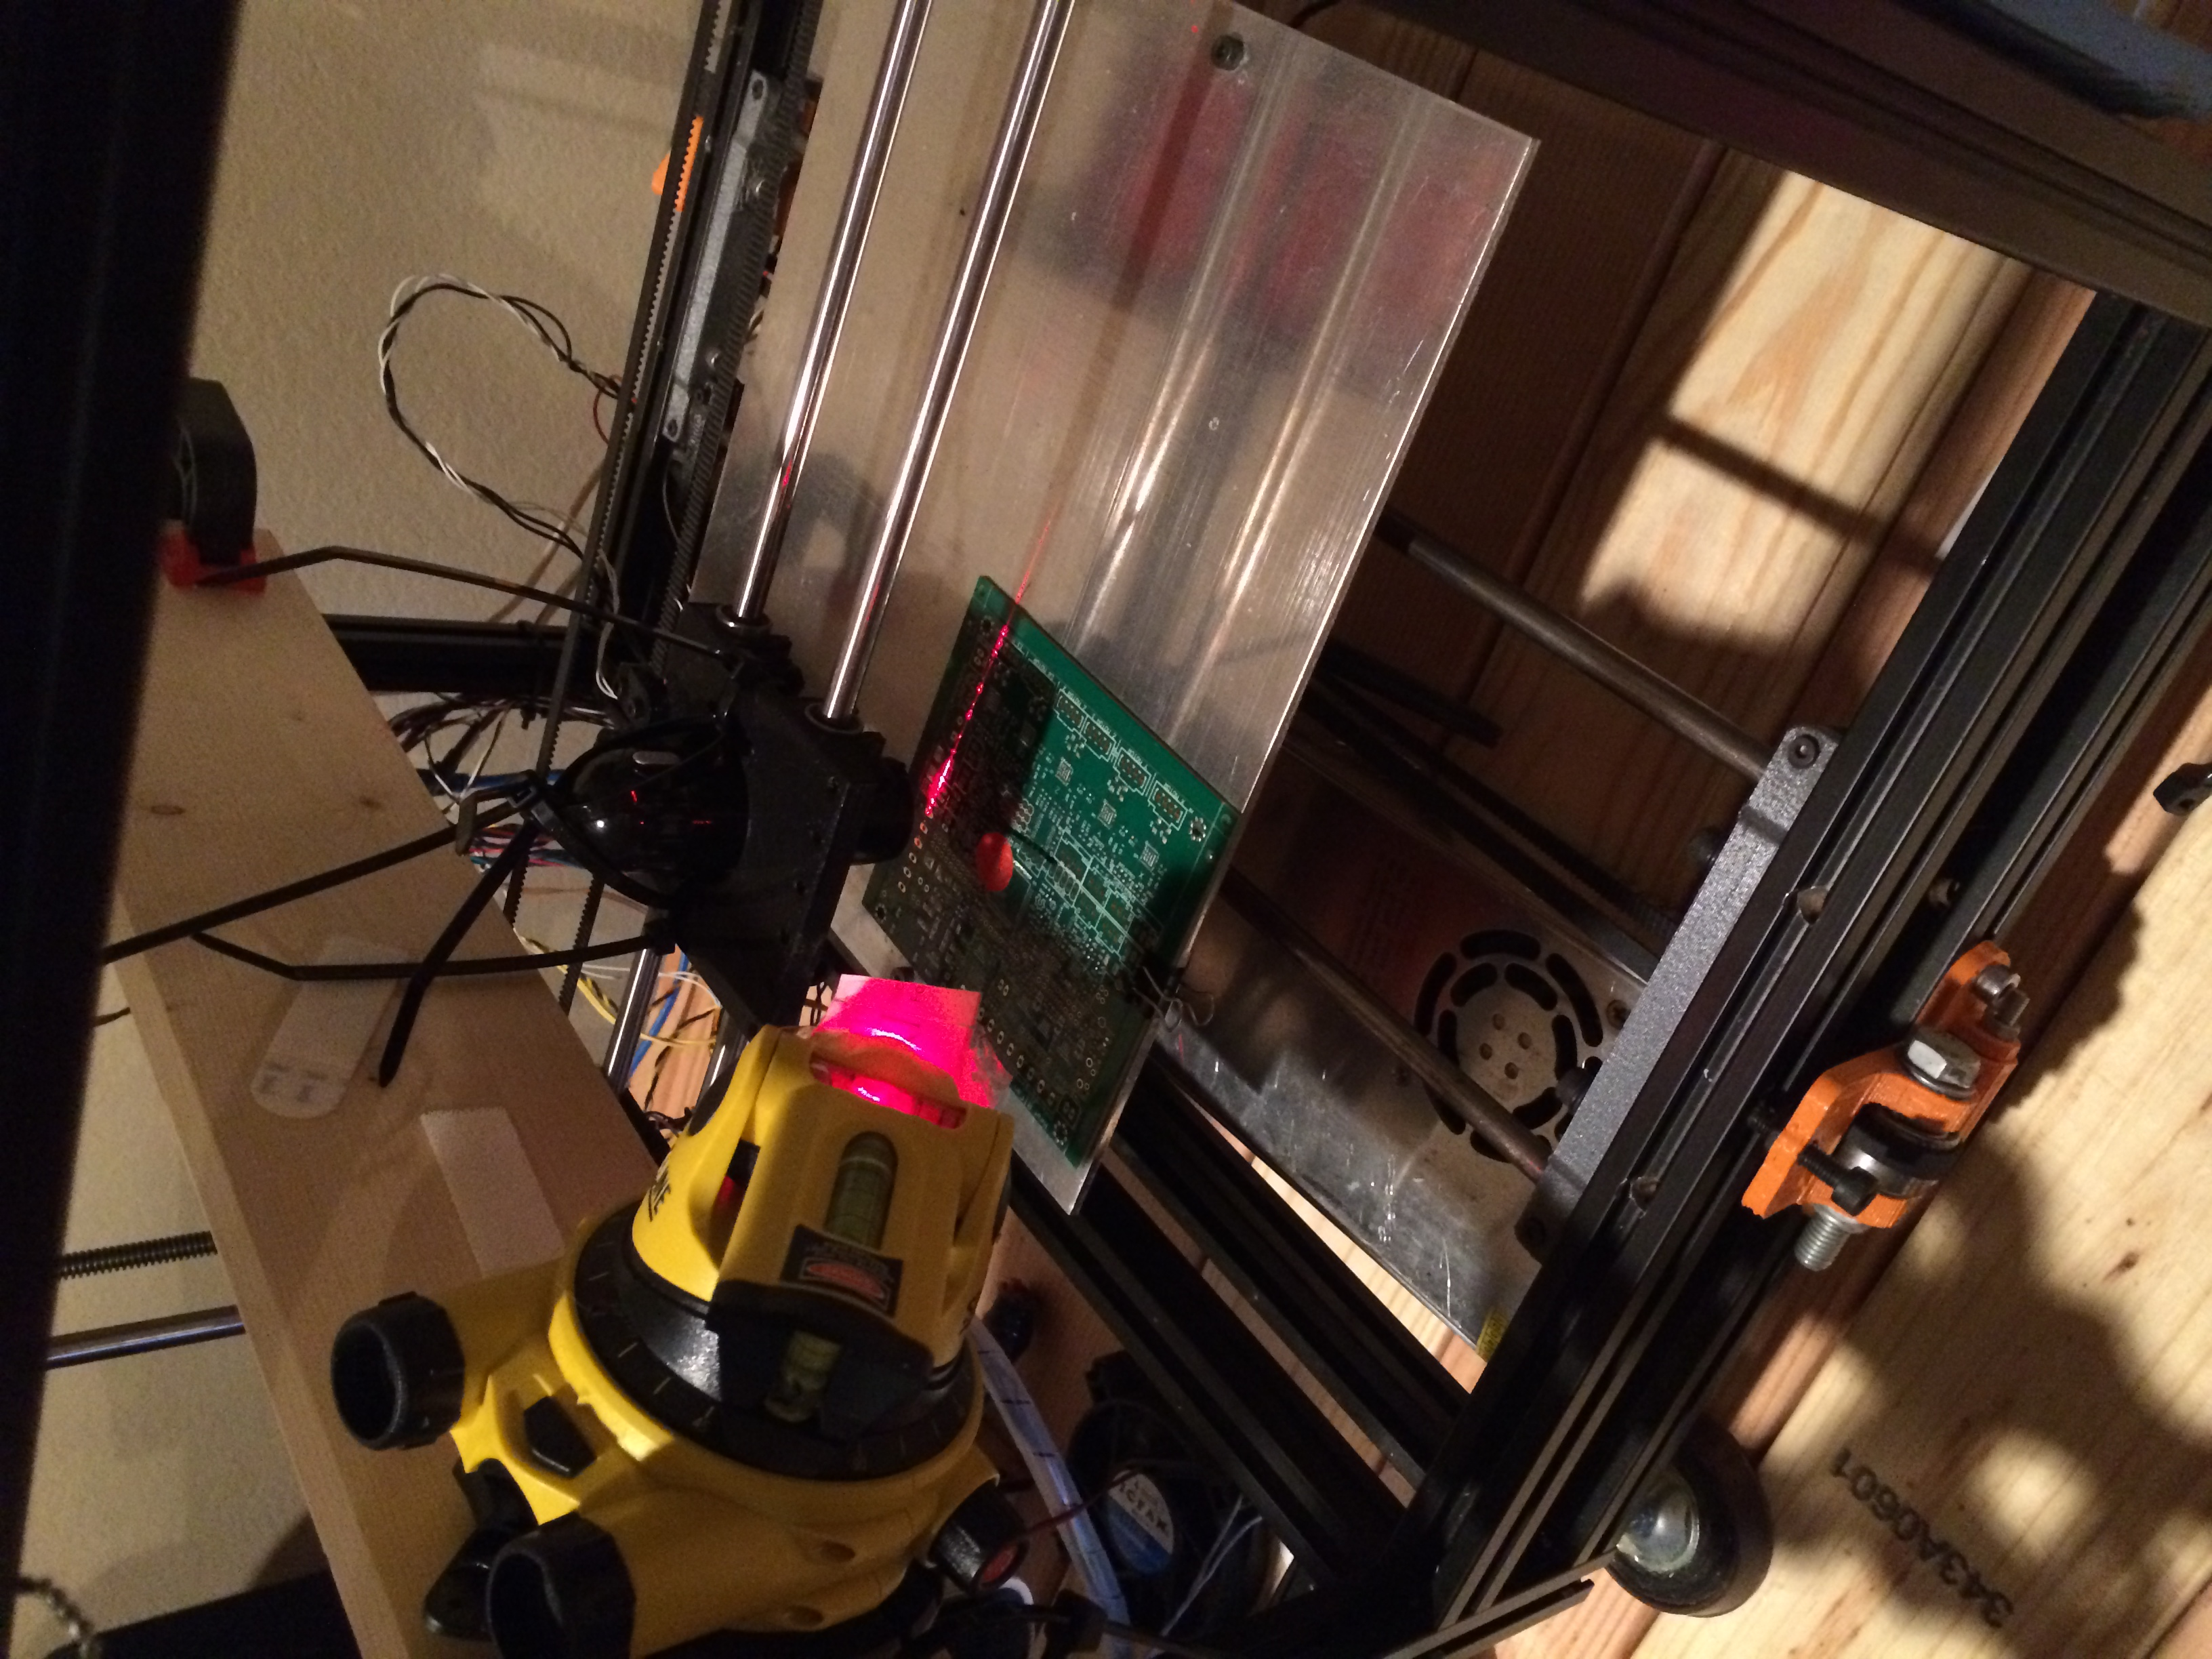
\includegraphics[scale=0.1,angle=270]{images/volume_analysis_setup/IMG_0605.JPG}
\newpage

%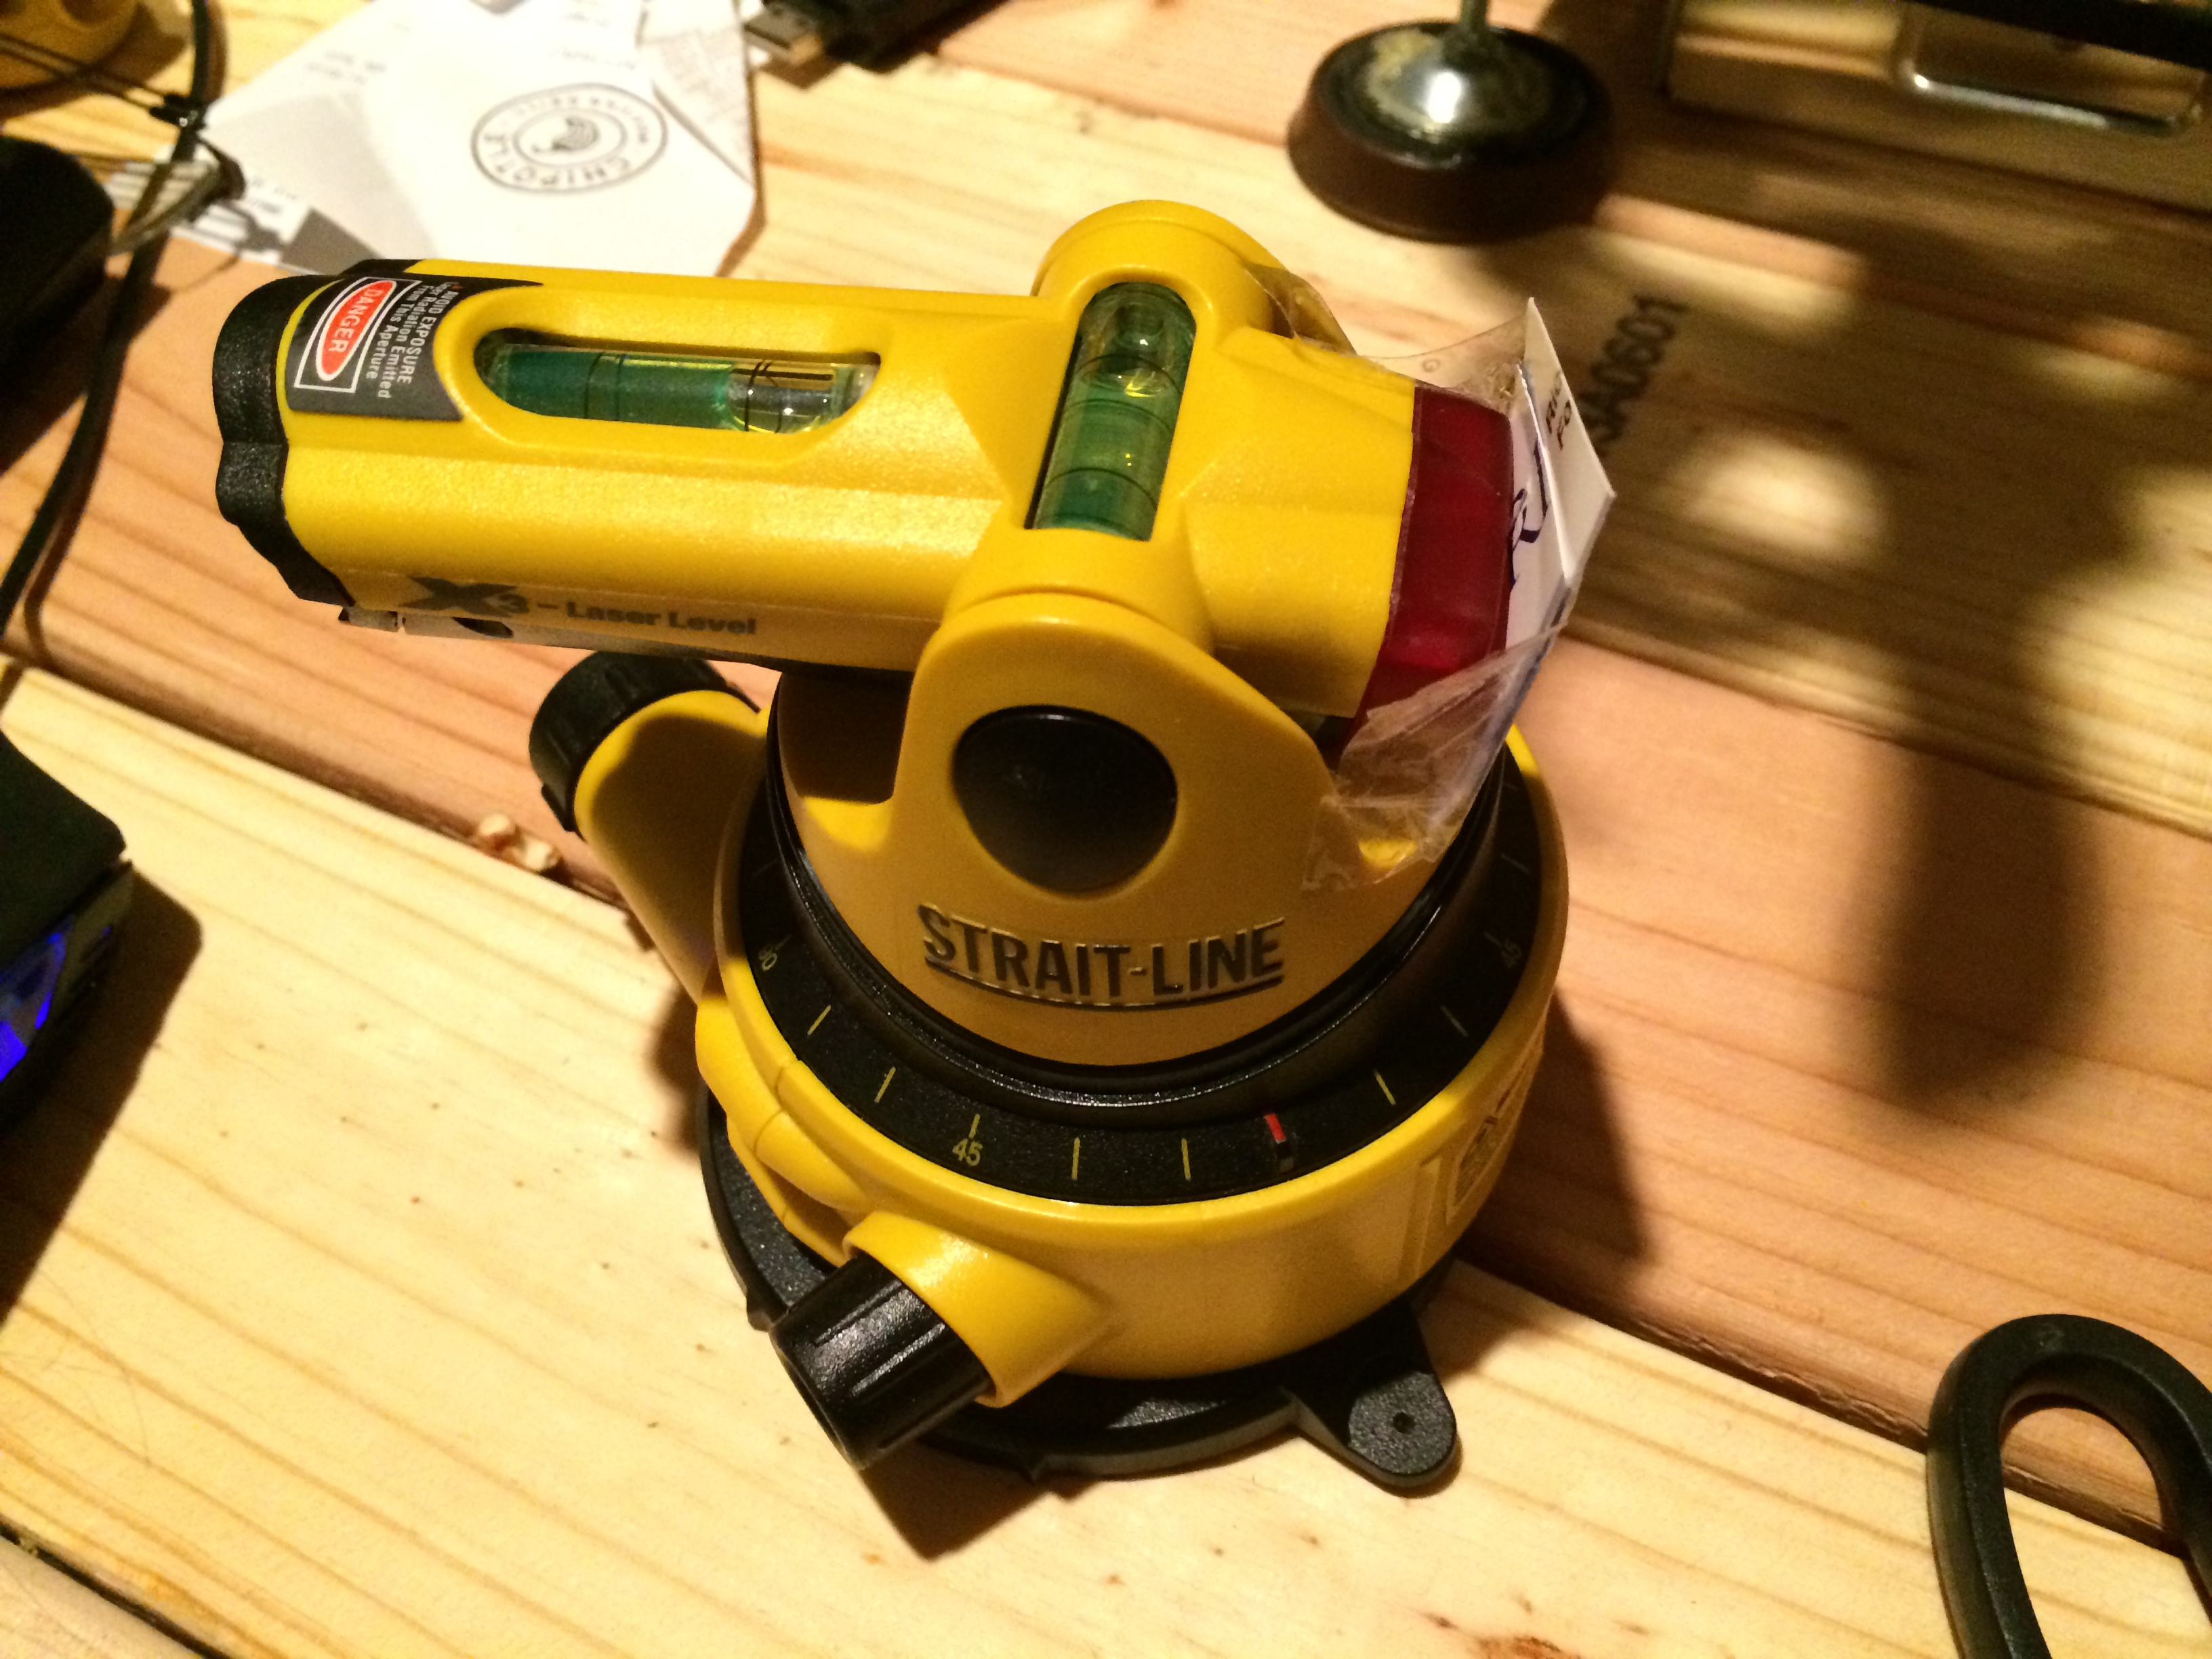
\includegraphics[scale=0.1,angle=270]{images/volume_analysis_setup/IMG_0607.JPG}
%\newpage
%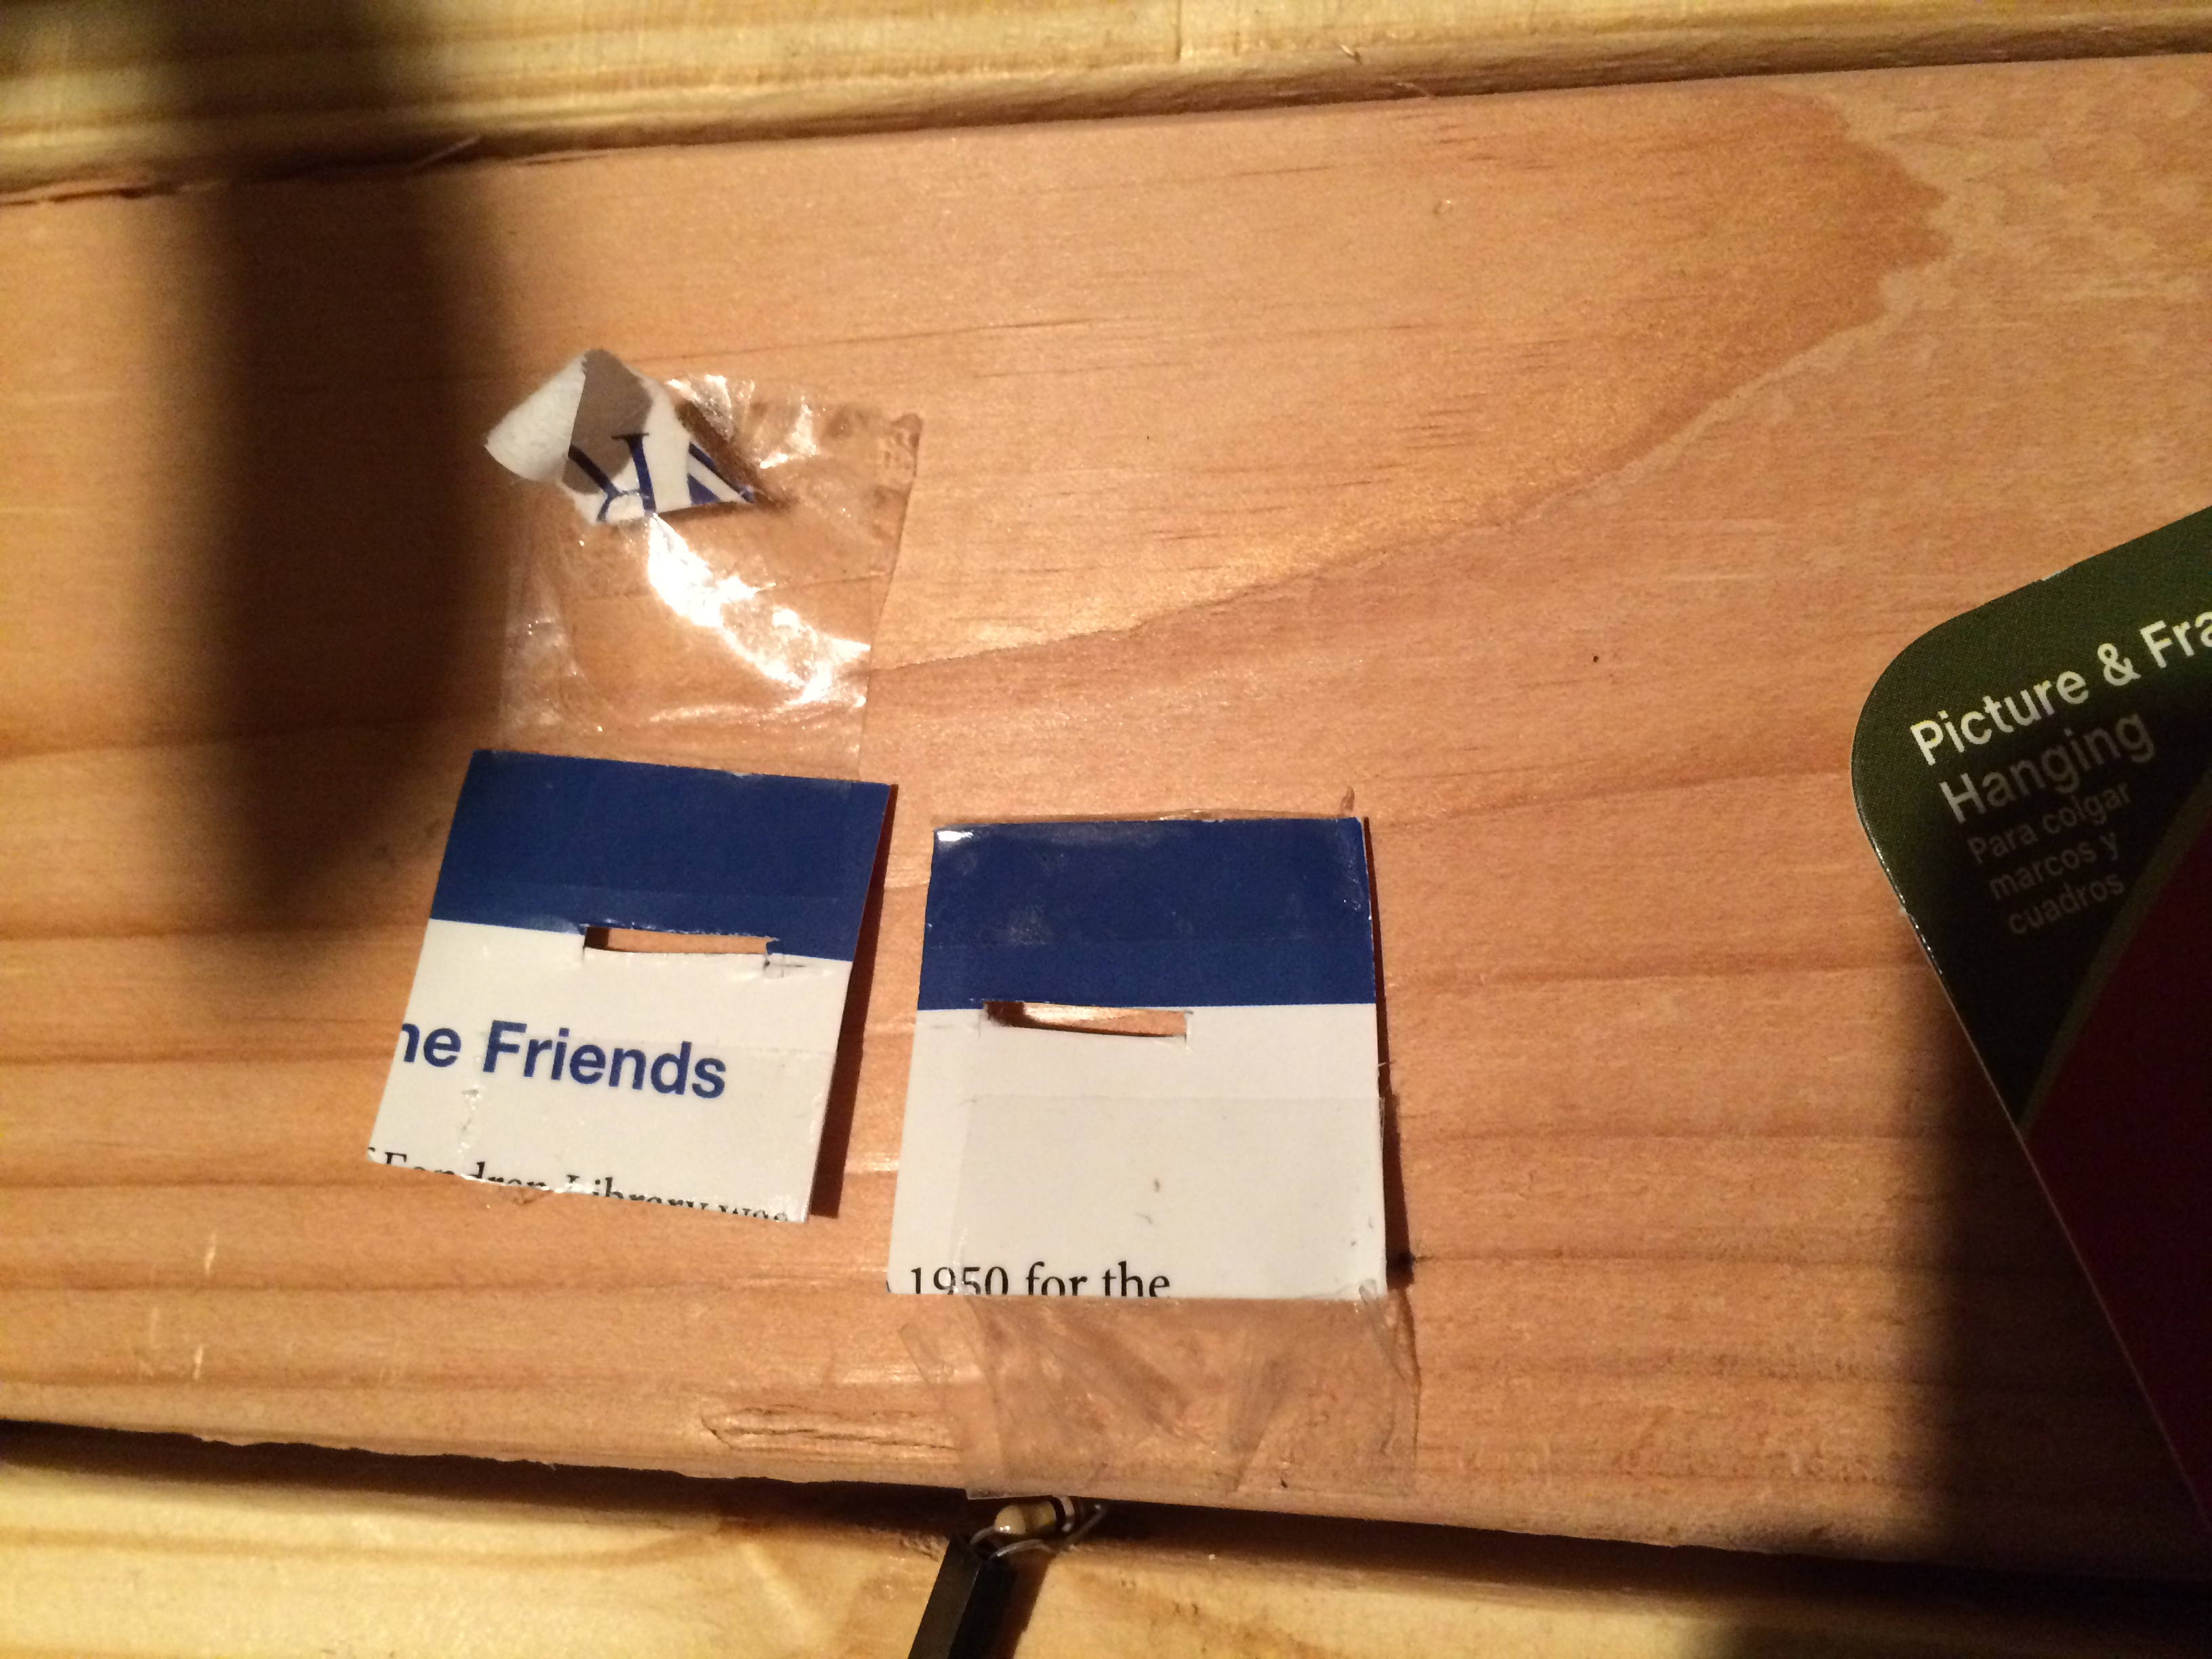
\includegraphics[scale=0.1,angle=270]{images/volume_analysis_setup/IMG_0608.JPG}
%\newpage
%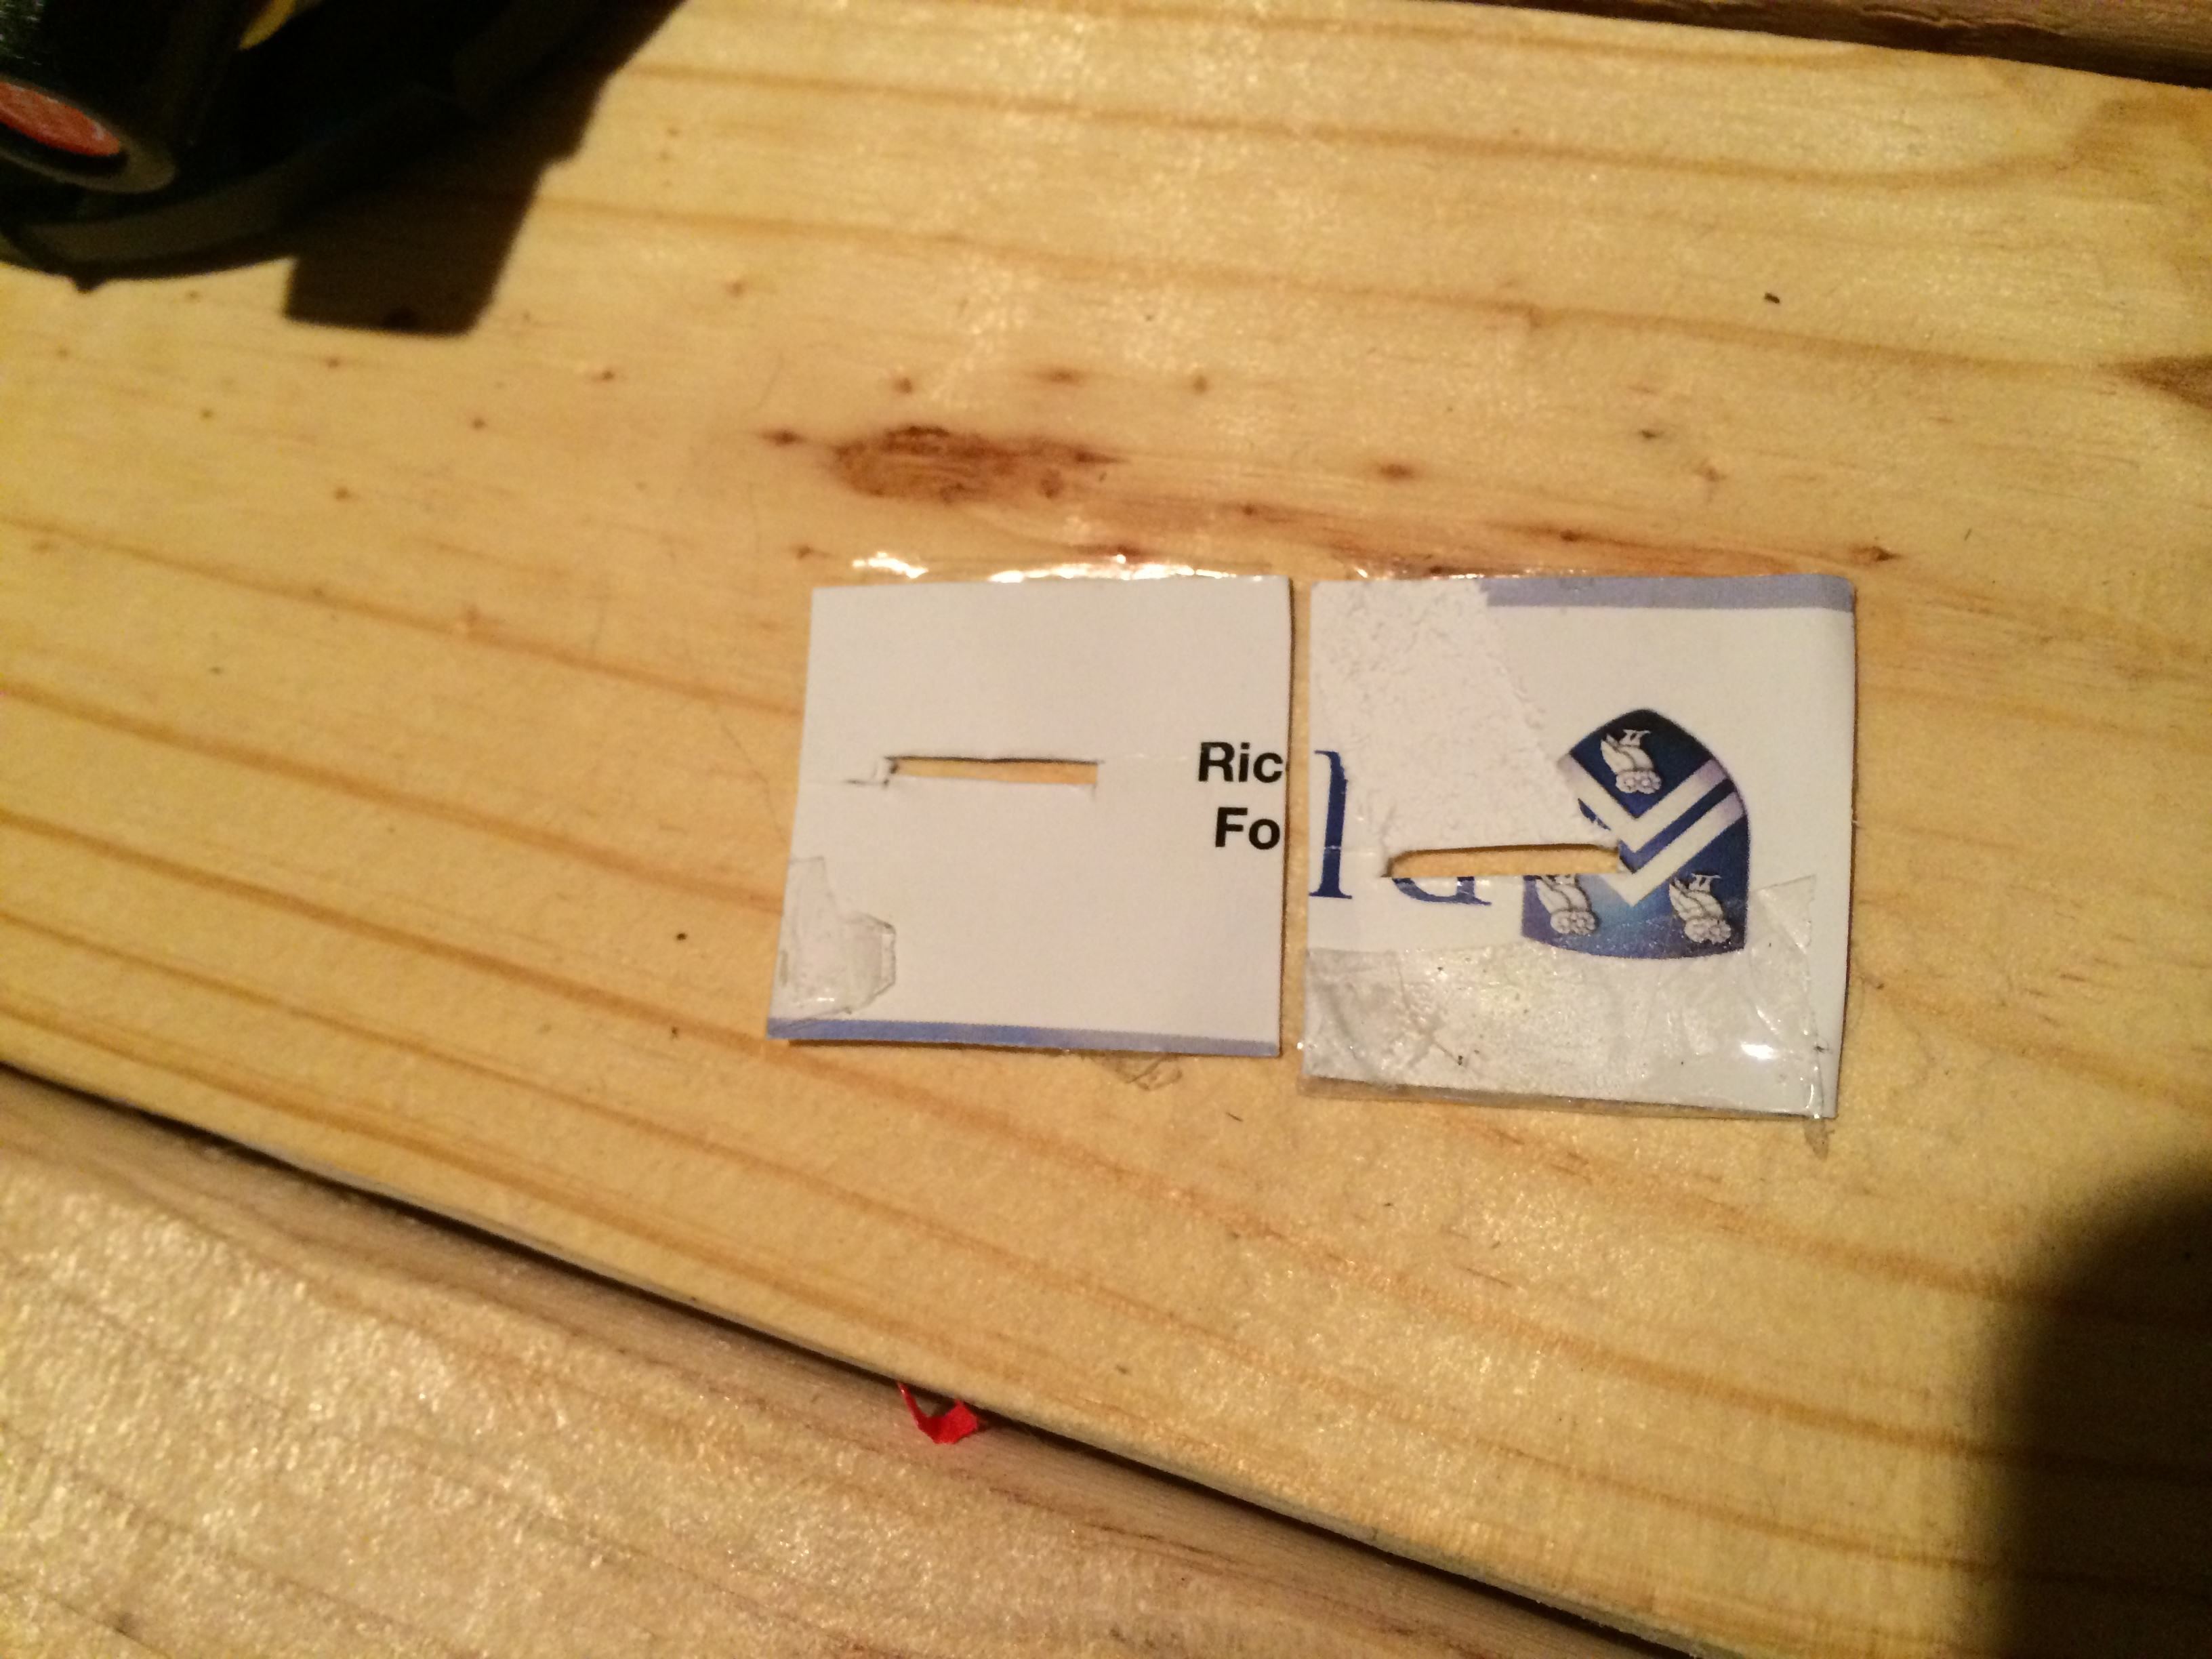
\includegraphics[scale=0.1,angle=270]{images/volume_analysis_setup/IMG_0609.JPG}
%\newpage
%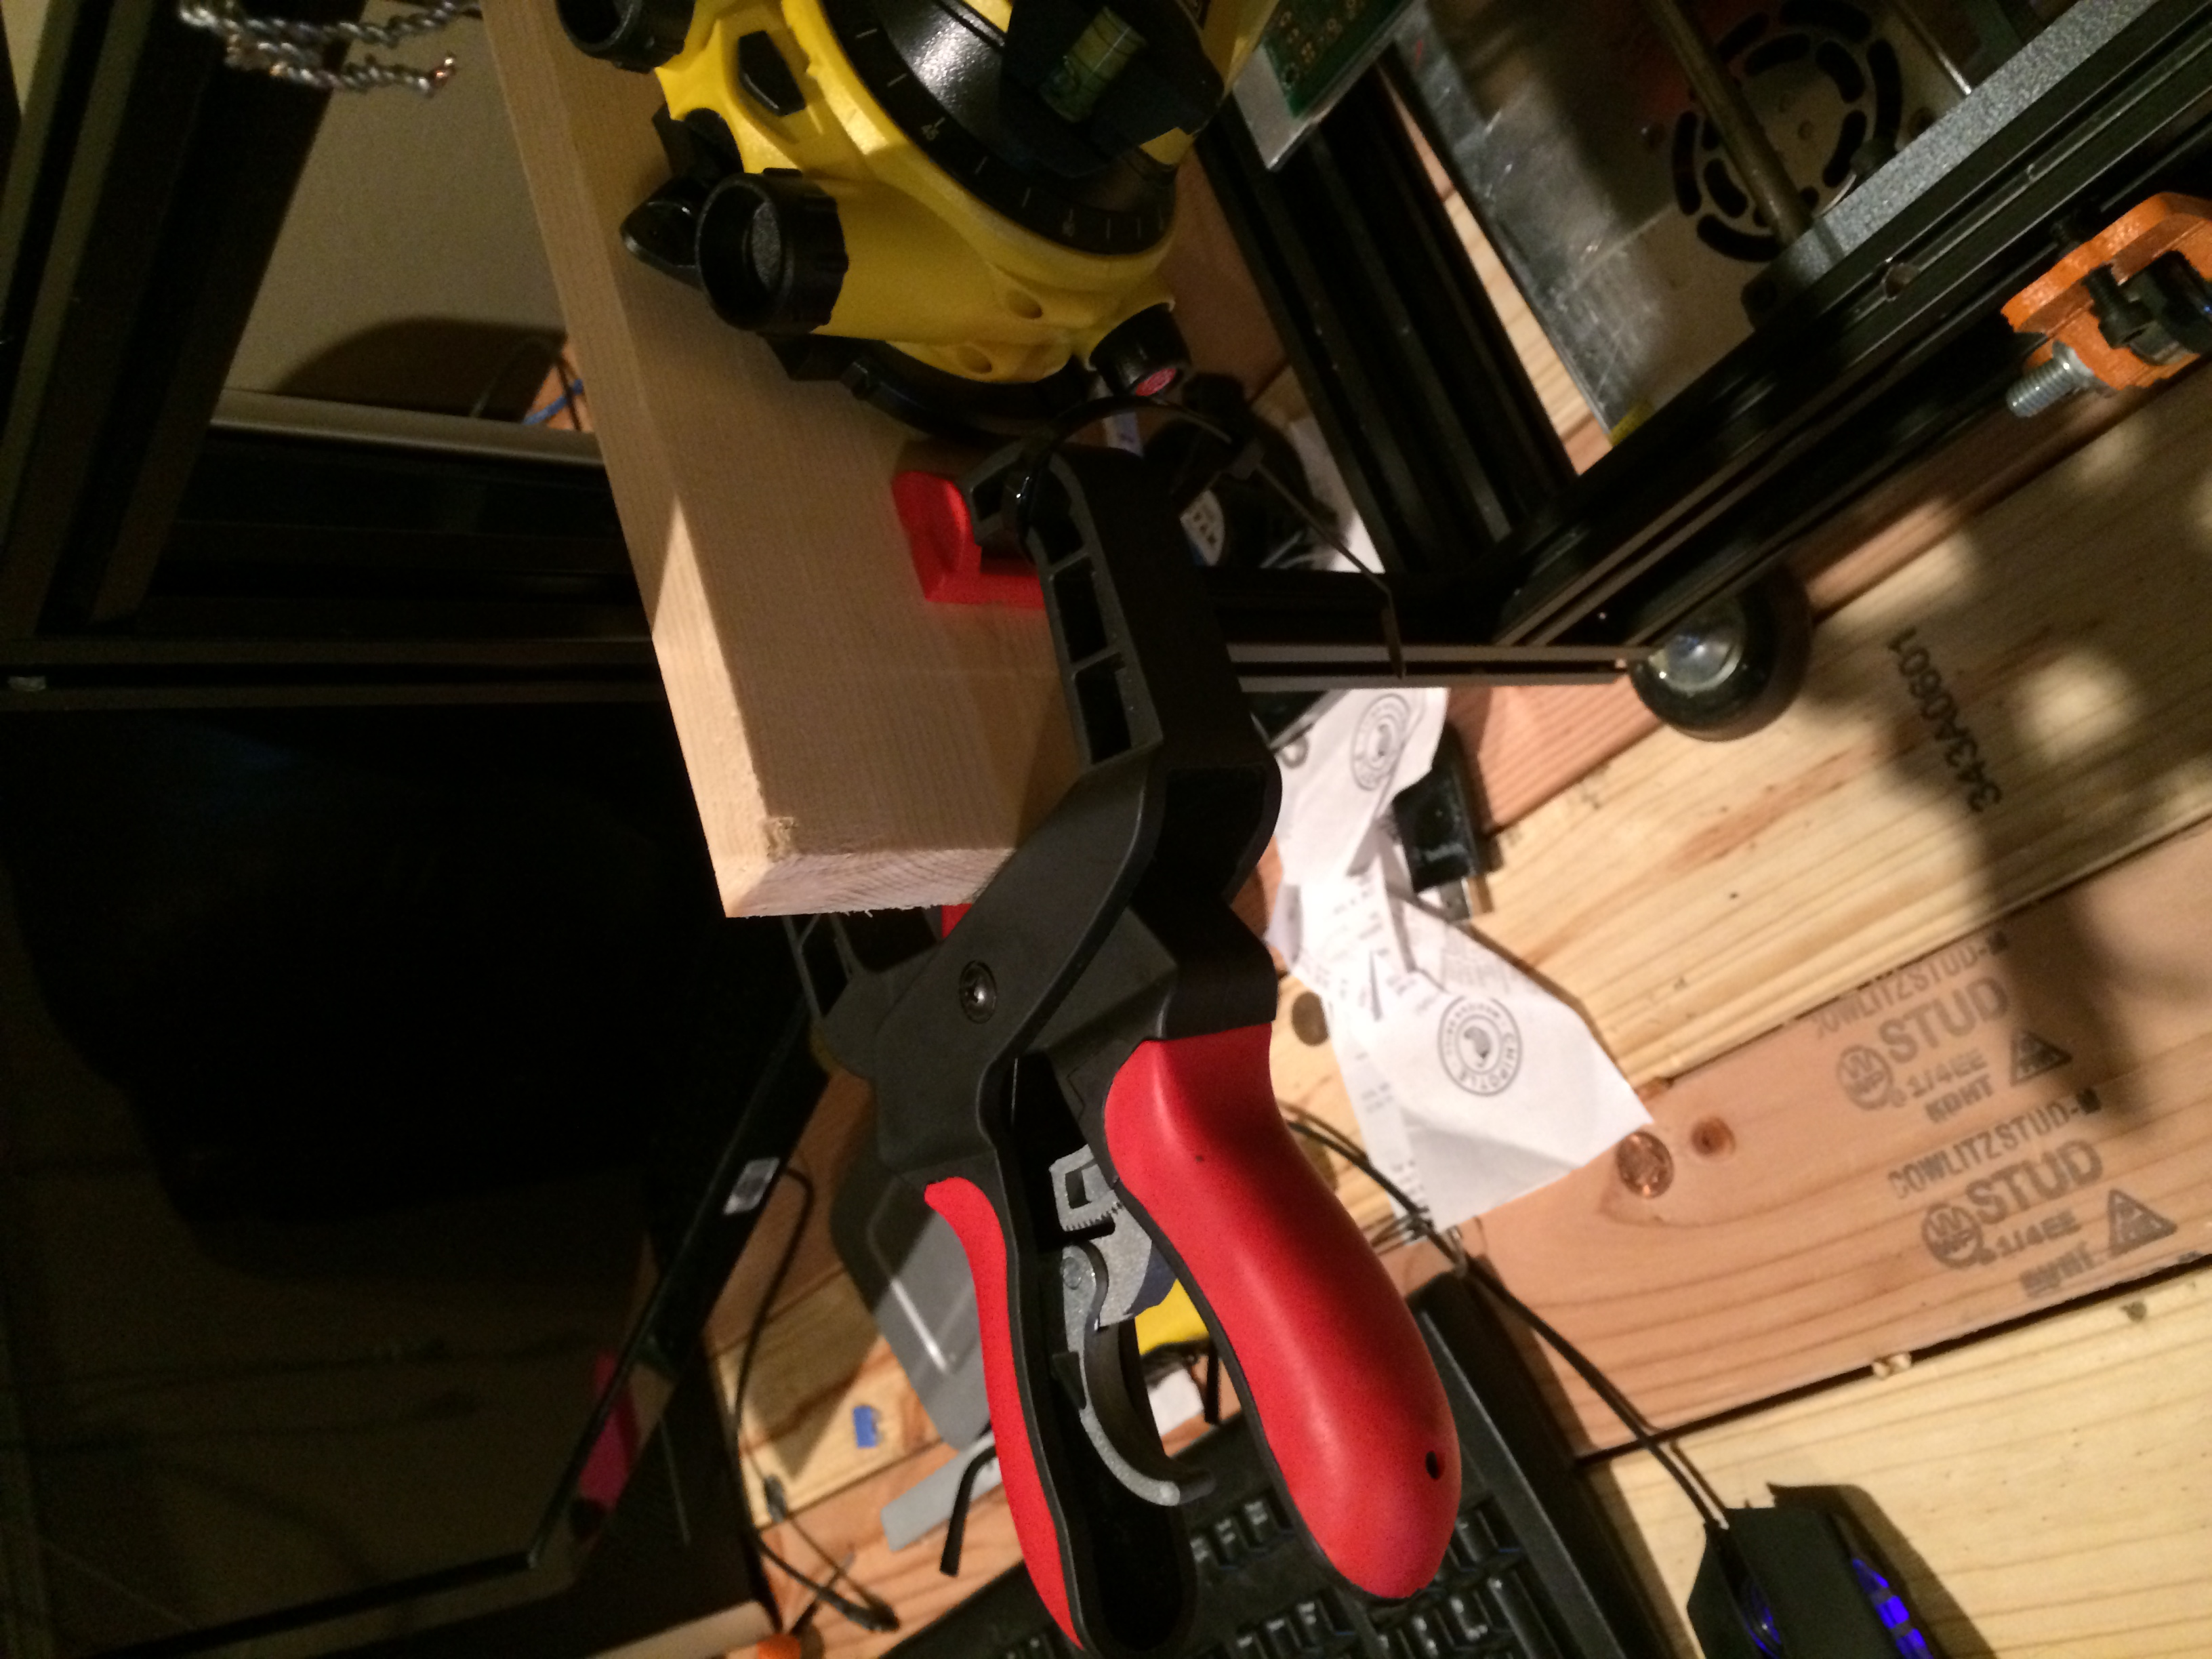
\includegraphics[scale=0.1,angle=270]{images/volume_analysis_setup/IMG_0610.JPG}
%\newpage






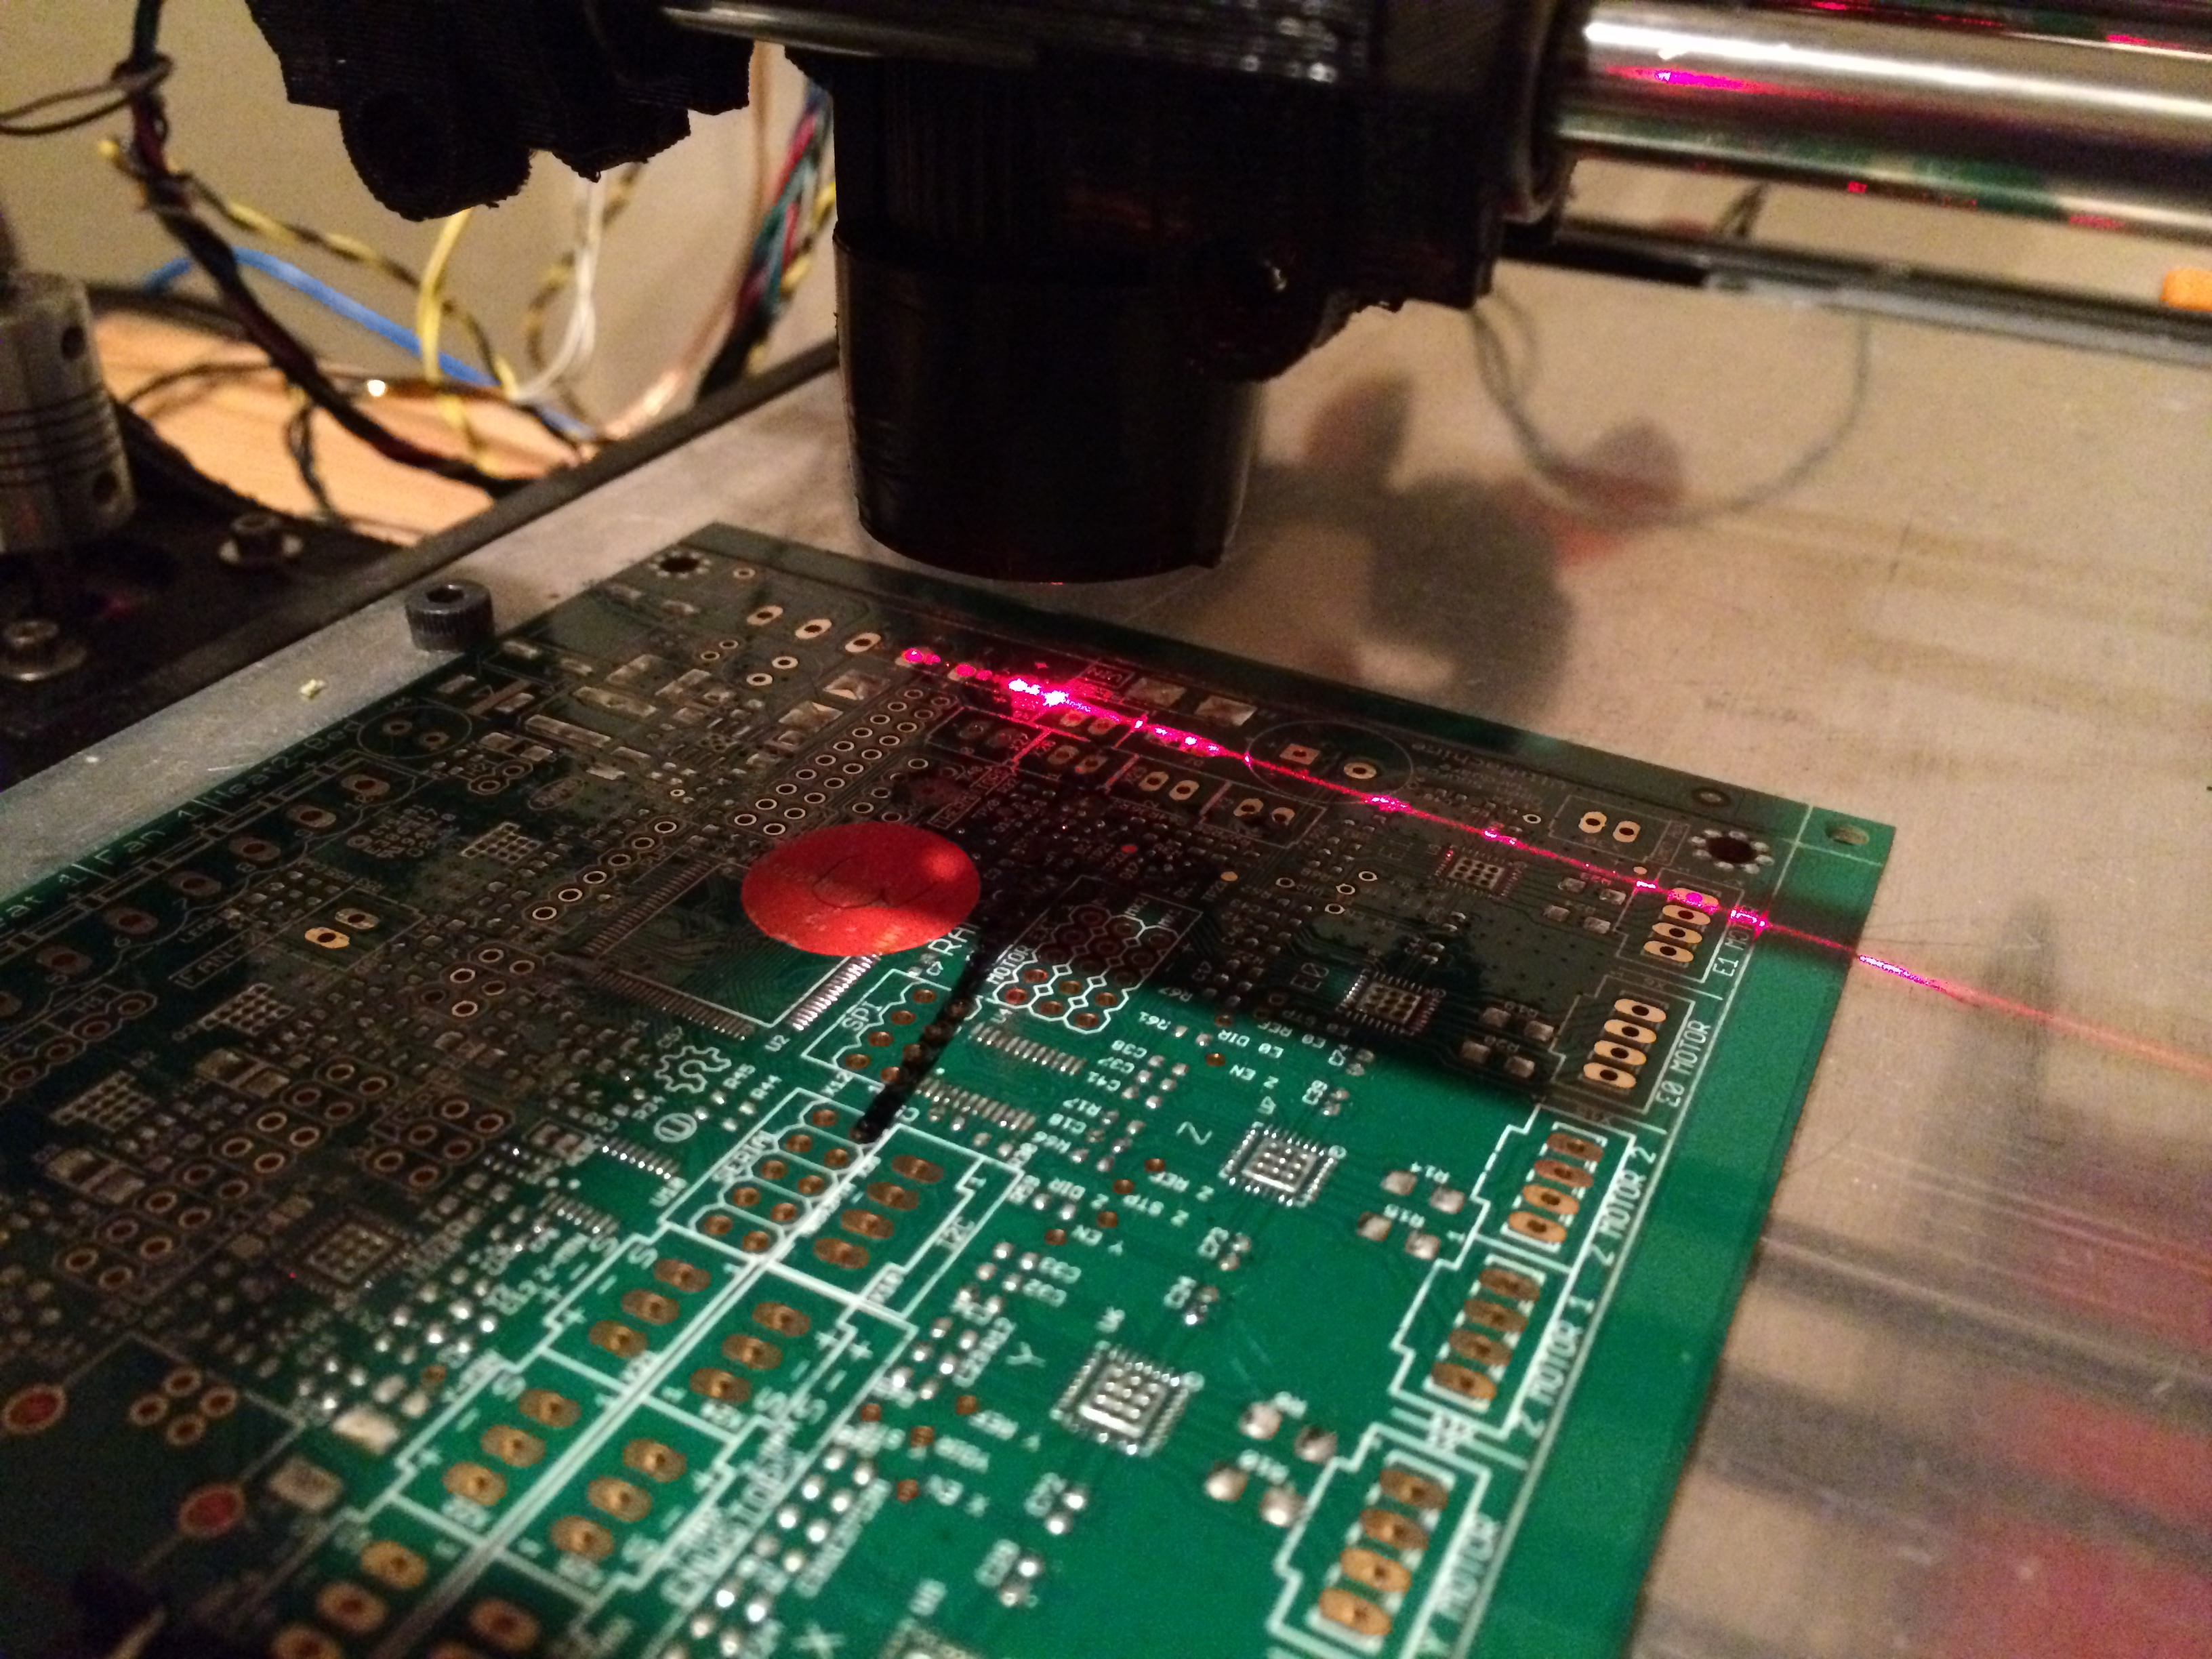
\includegraphics[scale=0.1]{images/volume_analysis_setup/IMG_0606.JPG}
\newpage

\includegraphics{images/volume_analysis_setup/laser-8}
\newpage

\section{Volume Image Processing}
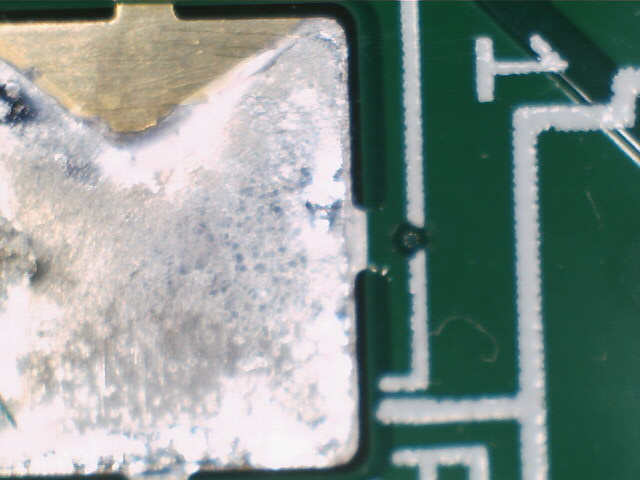
\includegraphics[scale=0.8]{images/volume_image_processing/led_image.png}
\newpage
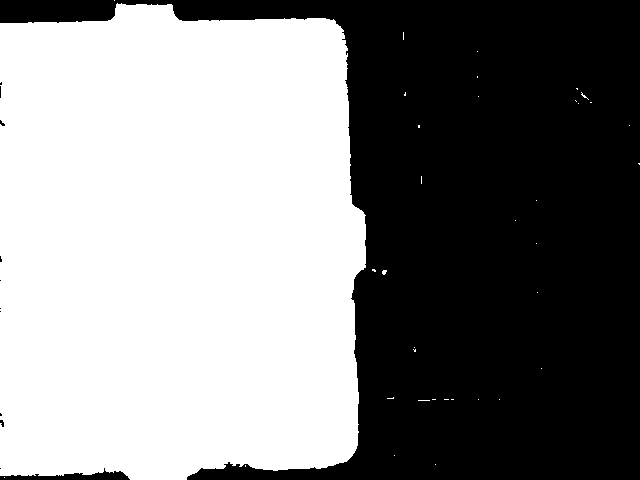
\includegraphics[scale=0.8]{images/volume_image_processing/binary_led_image.png}
\newpage
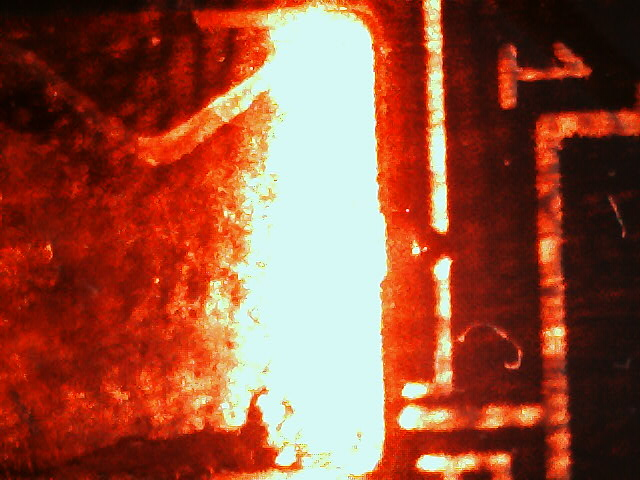
\includegraphics[scale=0.8]{images/volume_image_processing/laser_image.png}
\newpage

\includegraphics[scale=0.8]{images/volume_image_processing/binary_laser_image.png}
\newpage
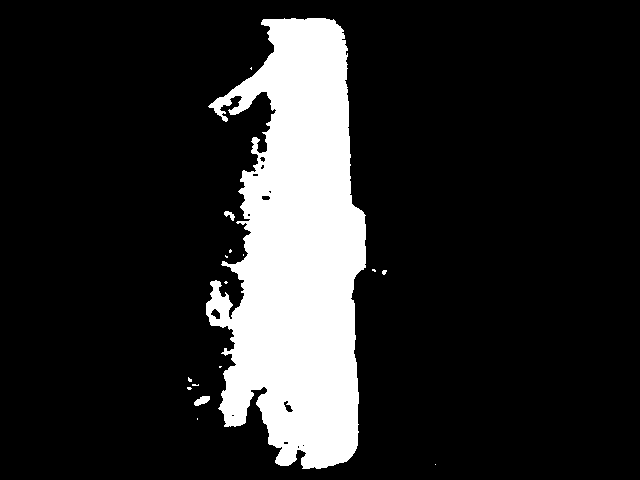
\includegraphics[scale=0.8]{images/volume_image_processing/union_laser_led_binaries.png}
\newpage

\section{Volume Results}
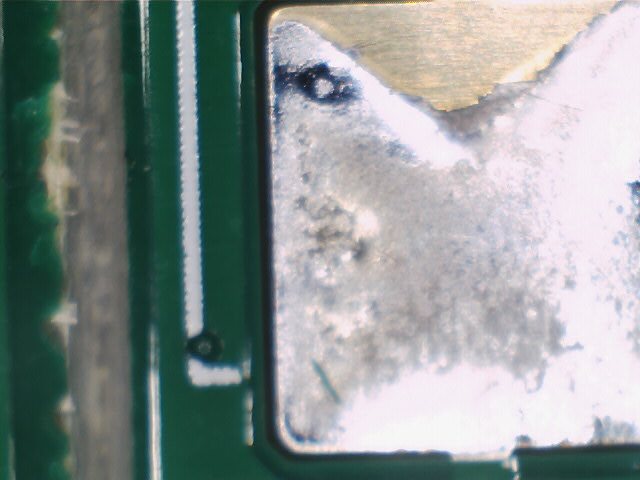
\includegraphics[scale=0.8]{images/volume_results/solder_led_hole.png}
\newpage
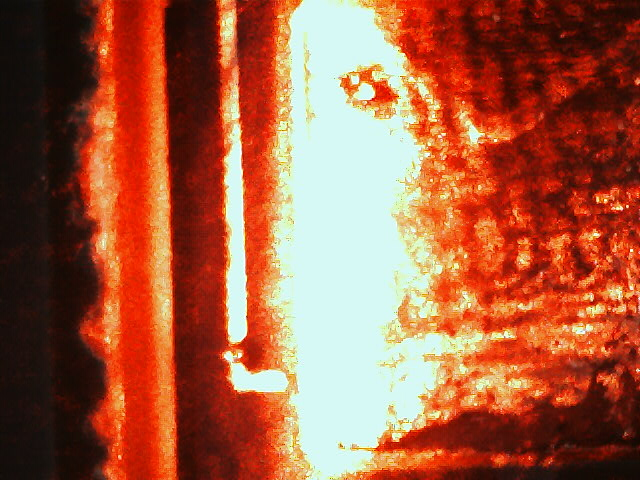
\includegraphics[scale=0.8]{images/volume_results/solder_laser_hole.png}
\newpage
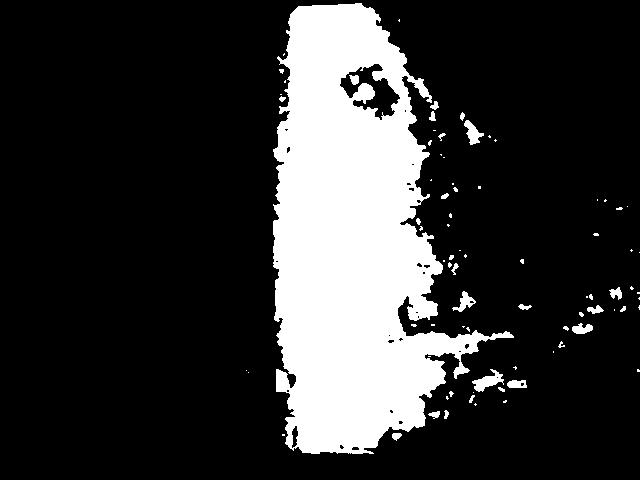
\includegraphics[scale=0.8]{images/volume_results/binary_image_hole.png}
Notice how the top of the white blob is thinner than the middle.  That is because the volume of solder at the top is less than the volume of solder at the middle. Also notice the black hole, this corresponds to a hole in the solder paste.
\newpage
\section{Classification}
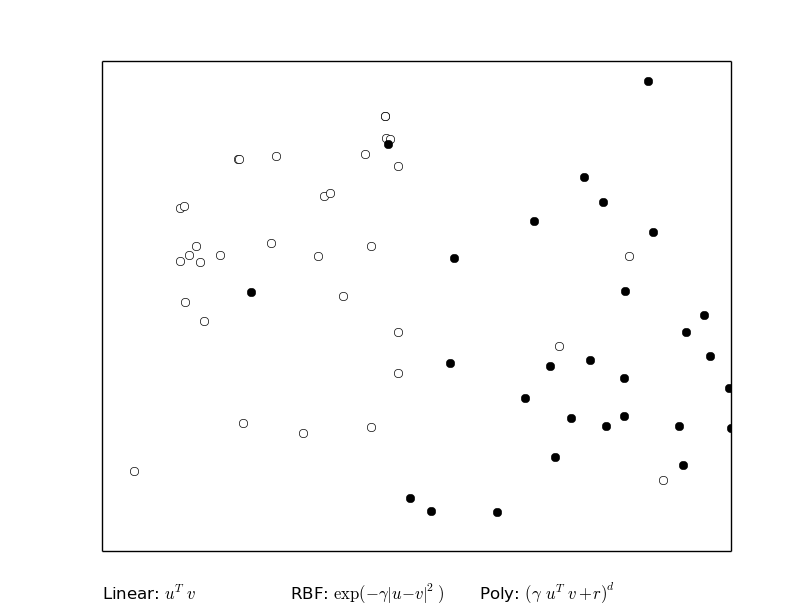
\includegraphics[scale=0.8]{images/Classification/data.png}
\newpage
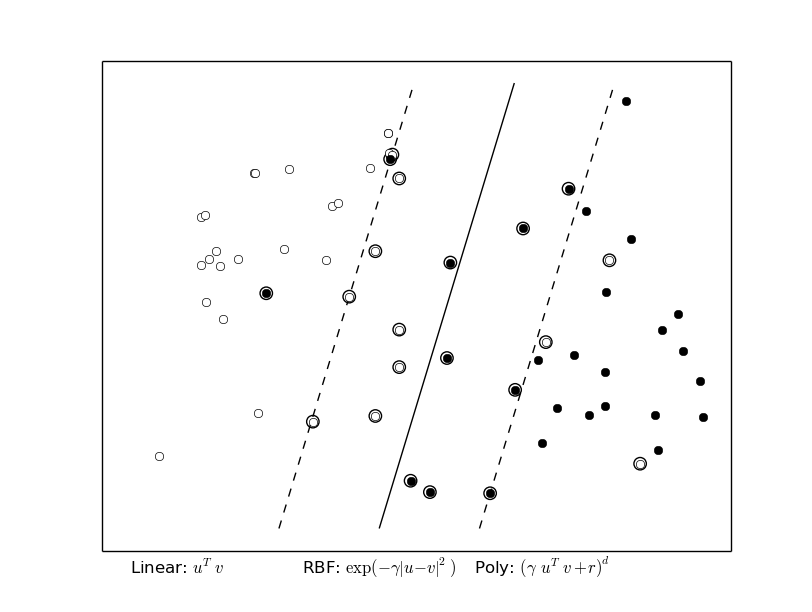
\includegraphics[scale=0.8]{images/Classification/analized_data.png}

%\begin{abstract}

%\end{abstract}


%\section{Introduction}
%Repeatability and accuracy is essential to PCB manufacturing.  That is why careful inspection %of PCB boards is an integral component of the PCB manufacturing process.  It is also essential %to 3D printing.  As 3D printing technology becomes more common place 

%\paragraph{Outline}
%The remainder of this article is organized as follows.
%Section~\ref{previous work} gives account of previous work.
%Our new and exciting results are described in Section~\ref{results}.
%Finally, Section~\ref{conclusions} gives the conclusions.

%\section{Previous work}\label{previous work}
%A much longer \LaTeXe{} example was written by Gil~\cite{Gil:02}.

%\section{Results}\label{results}
%In this section we describe the results.

%\section{Conclusions}\label{conclusions}
%We worked hard, and achieved very little.

%\bibliographystyle{abbrv}
%\bibliography{main}

\end{document}
